\section{Evaluation}
\label{sec:evaluation}
\todo{Improve naming algorithms to new names we selected}
\todo{Here outline also why we evaluate the benchmark this way, why this is a proxy for a useful benchmark
and then repeat again: no emperical data.}

We evaluate our benchmark using a scale 0.1 SolidBench dataset 
(158,233 RDF files, 1,531 vaults, 3,556,159 triples). 
Using the default hyperparameters in Table~\ref{tab:generation_hyperparameters}, 
we generate 8 sequences totaling 192 queries. 
These queries are from the interactive workload, are split into discover and short queries,
with multiple templates belonging to either of these groups.
Experiments run on an Ubuntu 20.04 machine (Intel Core i5-9400) 
with 16 GB RAM allocated to the engine and a 180-second query timeout. 
We repeat each sequence 10 times to minimize variance and 
inject a uniform 70–90 ms latency to simulate a realistic network environment.
The cache is scoped for a sequence, meaning no cache-state is shared between different executions or repetitions of
sequences.

% Outline the experimental setup, including machine scale and configurations. 
% State the primary aim: validating the benchmark. 
% Explain that validation relies on proxy metrics measuring data locality 
% (unique sources, cache hit rates, execution time) to demonstrate how 
% sequence design choices impact engine performance.
% Summarize our evaluation approach, which includes a holistic evaluation of benchmark characteristics, then
% a detailed analysis of logical session and interest modeling, refinement patterns, 
% and a comparison to alternative evaluation methods.

\subsection{Holistic Evaluation of Benchmark Characteristics}

First, we present the overall performance characteristics of the tested caching algorithms on the default configuration
of our introduced benchmark.

\paragraph{Unindexed LRU Cache}

In Figure~\ref{fig:unindexed-lru-cache-performance}, we find that the unindexed LRU cache reliably improves performance 
across all cache sizes, with larger caches yielding better results.
For total execution time of queries, the large cache is significantly better than the smaller cache sizes, while for
throughput the difference is less pronounced.

\begin{figure*}[t]
    \centering
    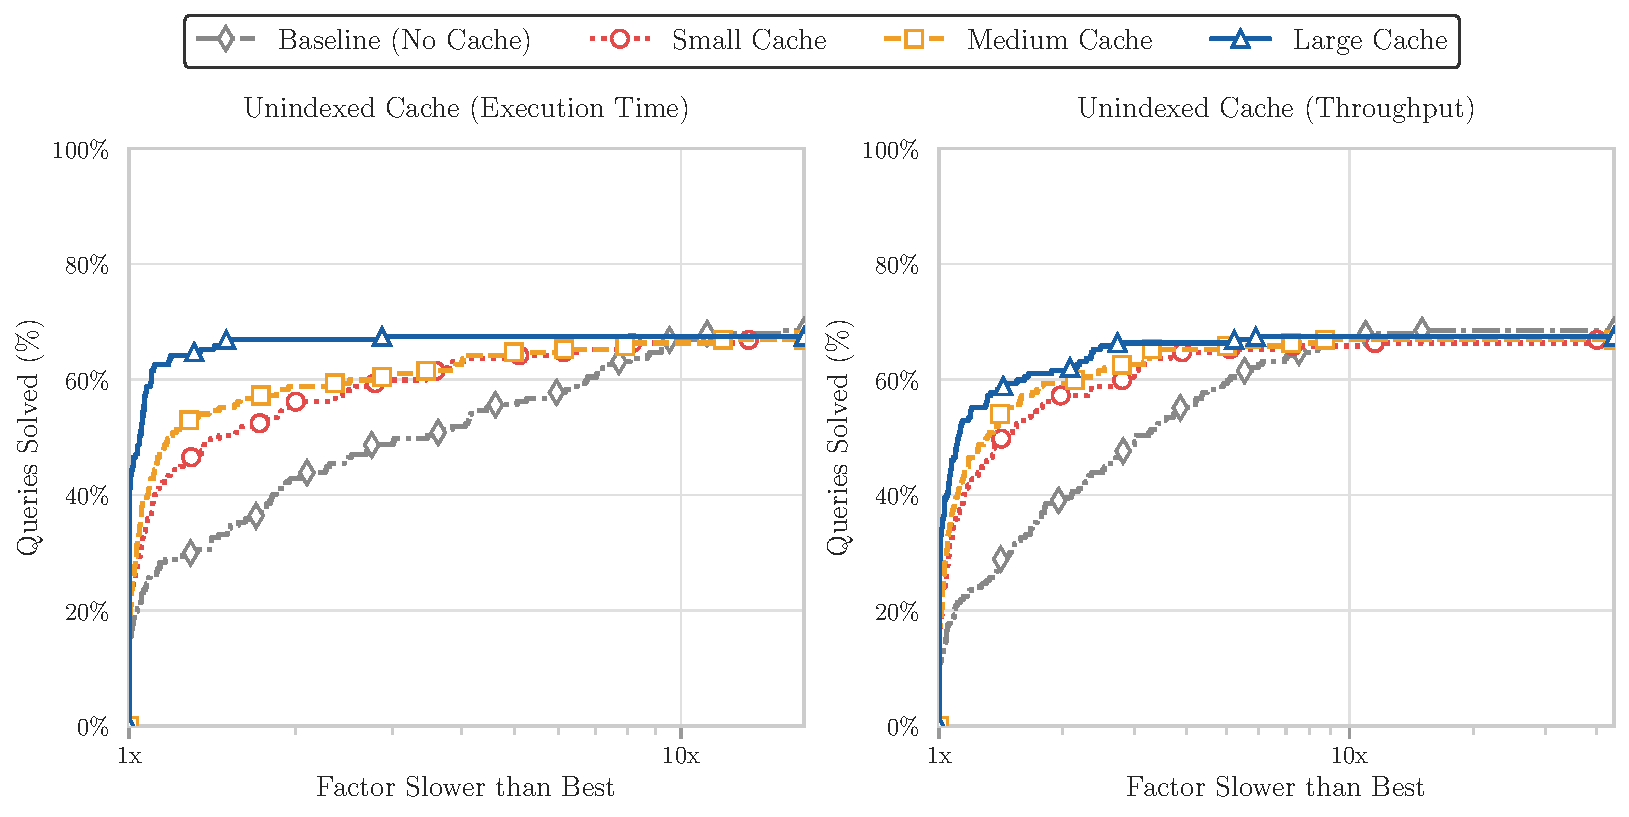
\includegraphics[width=\linewidth]{figures/performance_profile_normal_sequences_unindexed.pdf}
    \caption{Performance profiles of the LRU-based unindexed triples cache. 
    The y-axis shows the percentage of queries executing within a factor (x-axis) of the fastest algorithm. 
    Curves closer to the top-left indicate better overall performance. 
    The y-intercept ($x=1$) shows how often an algorithm is the outright fastest, 
    while the rightward trajectory demonstrates robustness 
    (e.g., $x=2, y=80\%$ means 80\% of queries execute within twice the fastest time).
    From the figure, we observe that all caching-based approaches outperform the no-cache baseline.}
    \label{fig:unindexed-lru-cache-performance}
\end{figure*}

\paragraph{Indexed LRU Cache}
As shown in Figure~\ref{fig:indexed-lru-cache-performance}, 
pre-indexing triples in the LRU cache accelerates successful query execution
but introduces higher initial overhead. 
When high cache eviction rates outweigh the efficiency gains of indexing, 
this ingestion cost slows down execution or causes timeouts. 
The figure illustrates this overhead, as the no-cache baseline ultimately solves a higher percentage 
of queries than the standard indexed cache as the line reaches a higher y-value. 

However, integrating cardinality estimation overcomes this limitation 
by enabling the query engine to generate more accurate query plans, 
increasing the percentage of solved queries and lowering execution times. 
Comparing the two estimation approaches, reachability-aware estimation 
outperforms reachability-agnostic estimation by ignoring irrelevant data. 
This effect is most pronounced in larger caches, where reachability-agnostic estimation 
yields only minor performance benefits, while reachability-aware estimation shows substantial improvements. 
This aligns with expectations: larger caches accumulate more irrelevant, 
out-of-context data, which the reachability-aware estimator successfully filters out.

\begin{figure*}[t]
    \centering
    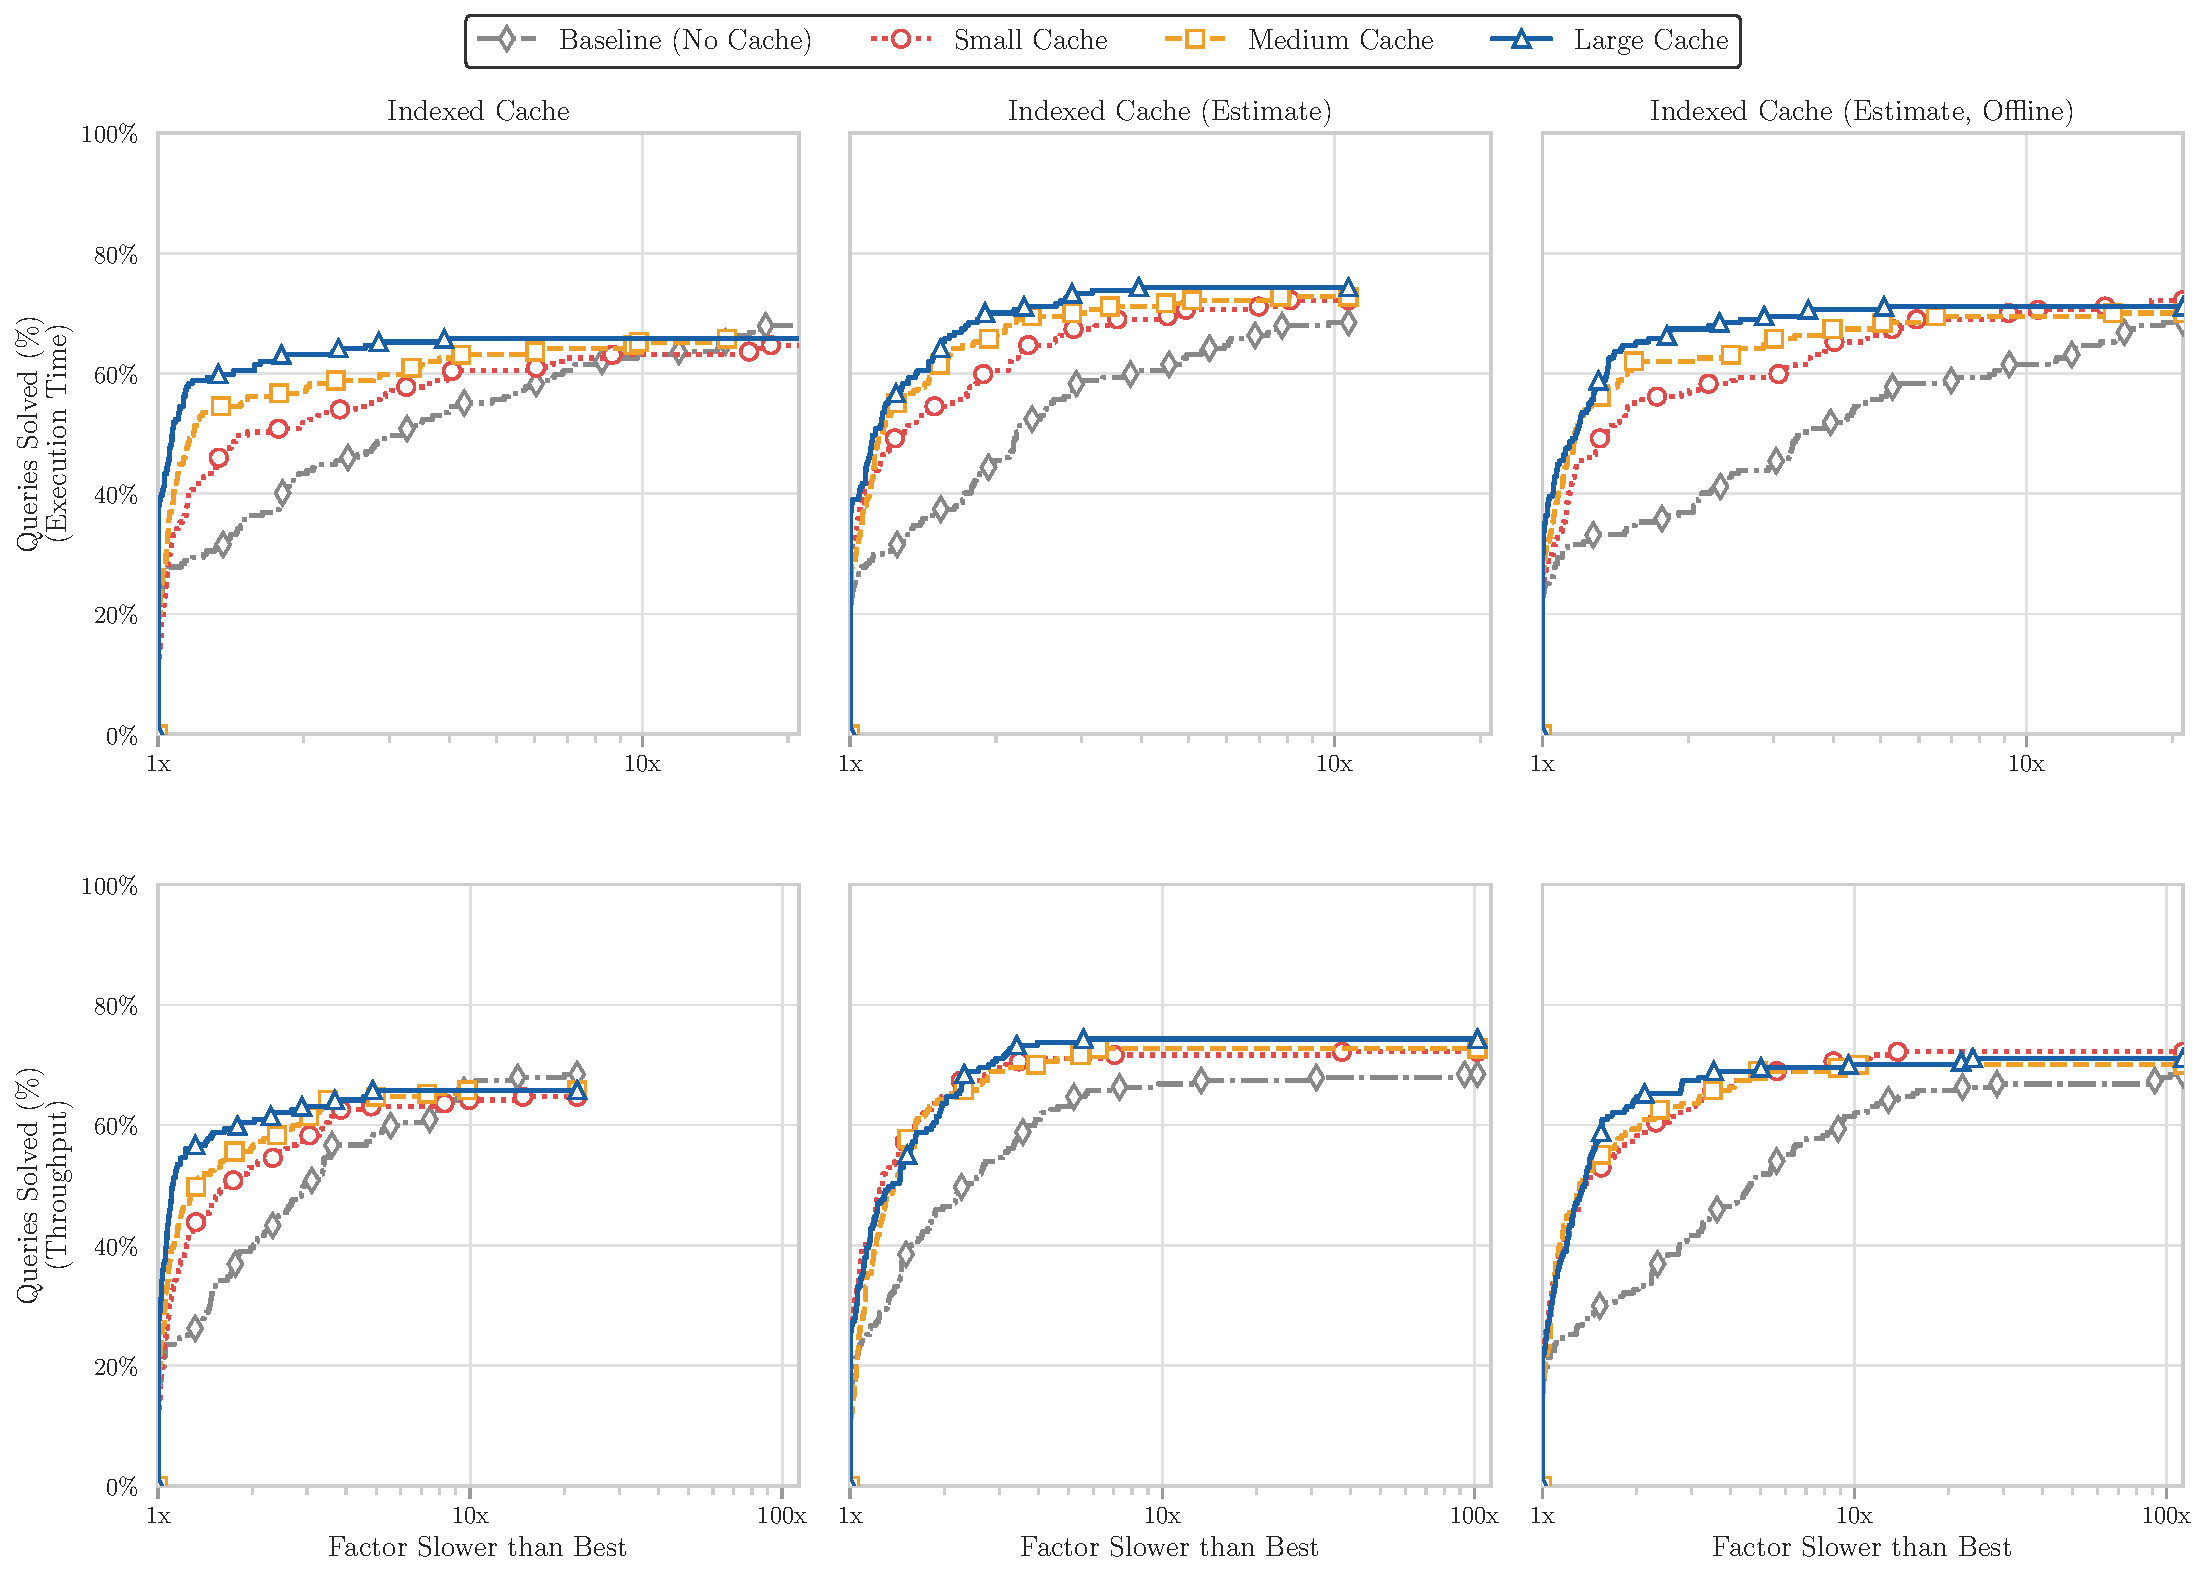
\includegraphics[width=\linewidth]{figures/performance_profile_normal_sequences_cache.pdf}
    \caption{Performance profiles of the LRU-based indexed cache family of algorithms. 
    The y-axis shows the percentage of queries executing within a factor (x-axis) of the fastest algorithm.}
    \label{fig:indexed-lru-cache-performance}
\end{figure*}


\paragraph{Memory-based Quad store Cache}
As shown in Figure~\ref{fig:quad-store-cache-performance}, 
the memory-based quad store cache exhibits high performance variance depending on the estimation strategy.
Without estimation (\textit{Indexed Store}), performance scales normally with capacity: 
the large cache achieves the best performance, while the medium and small caches sit lower 
but still reliably outperform the baseline. 
Similar to the LRU-based indexed cache, the baseline solves slightly more queries, indicating that the
performance overhead can cause query failures.
However, introducing online cardinality estimation (\textit{Indexed Store (Estimate)}) 
completely inverts the performance scaling observed without estimation, 
with the small and medium caches outperforming the large cache. 

The scaling nature of the performance penalty of cache size in estimation indicates that
executing count queries scales unfavorably as the cached quad store size increases.
Compared to the LRU-cache, which executes count triple pattern queries over small sources,
the quad store-based approach uses triple pattern queries over the entire quad store, but with
the graph term filled in to represent the current document.
For reachability-aware estimation the performance hit is not as big, especially in the
total execution time case.

\begin{figure*}[t]
    \centering
    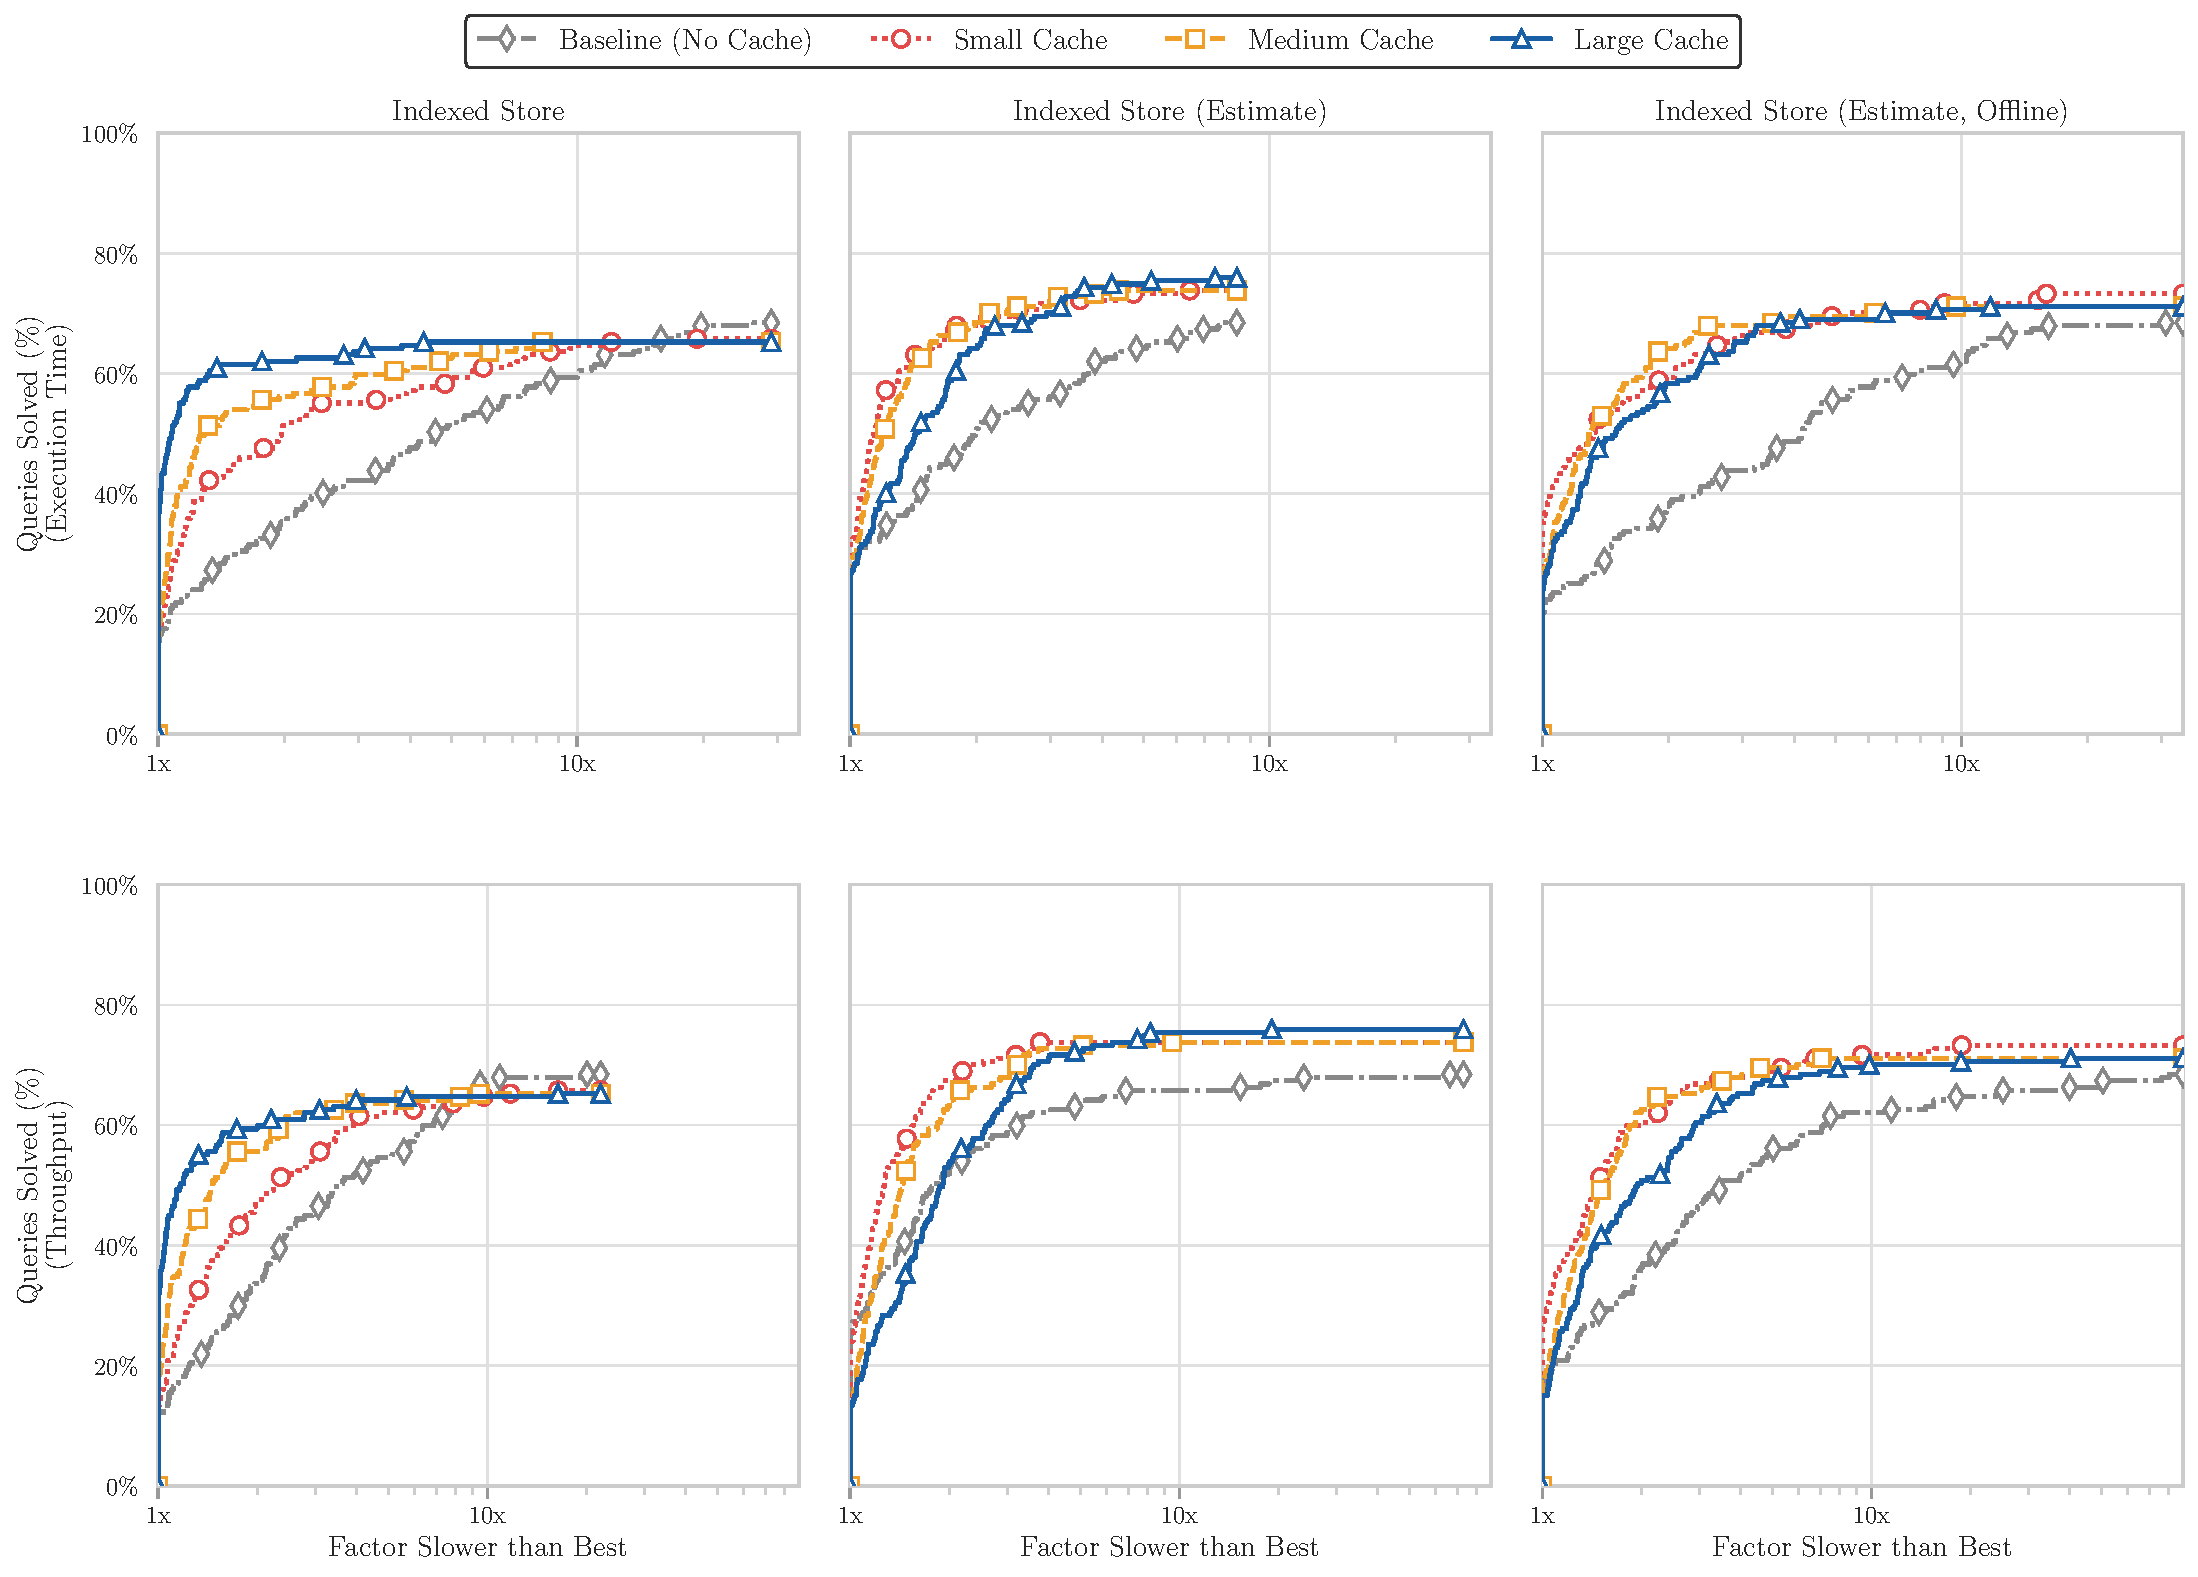
\includegraphics[width=\linewidth]{figures/performance_profile_normal_sequences_store.pdf}
    \caption{Performance profiles of the in-memory quad store cache family of algorithms. 
    The y-axis shows the percentage of queries executing within a factor (x-axis) of the fastest algorithm.}
    \label{fig:quad-store-cache-performance}
\end{figure*}

\paragraph{Disk-based Quad store Cache}

In Figure~\ref{fig:disk-store-cache-performance}, we see that the disk-based quad store cache performs....
\todo{PLACEHOLDER FIGURE}
\begin{figure*}[t]
    \centering
    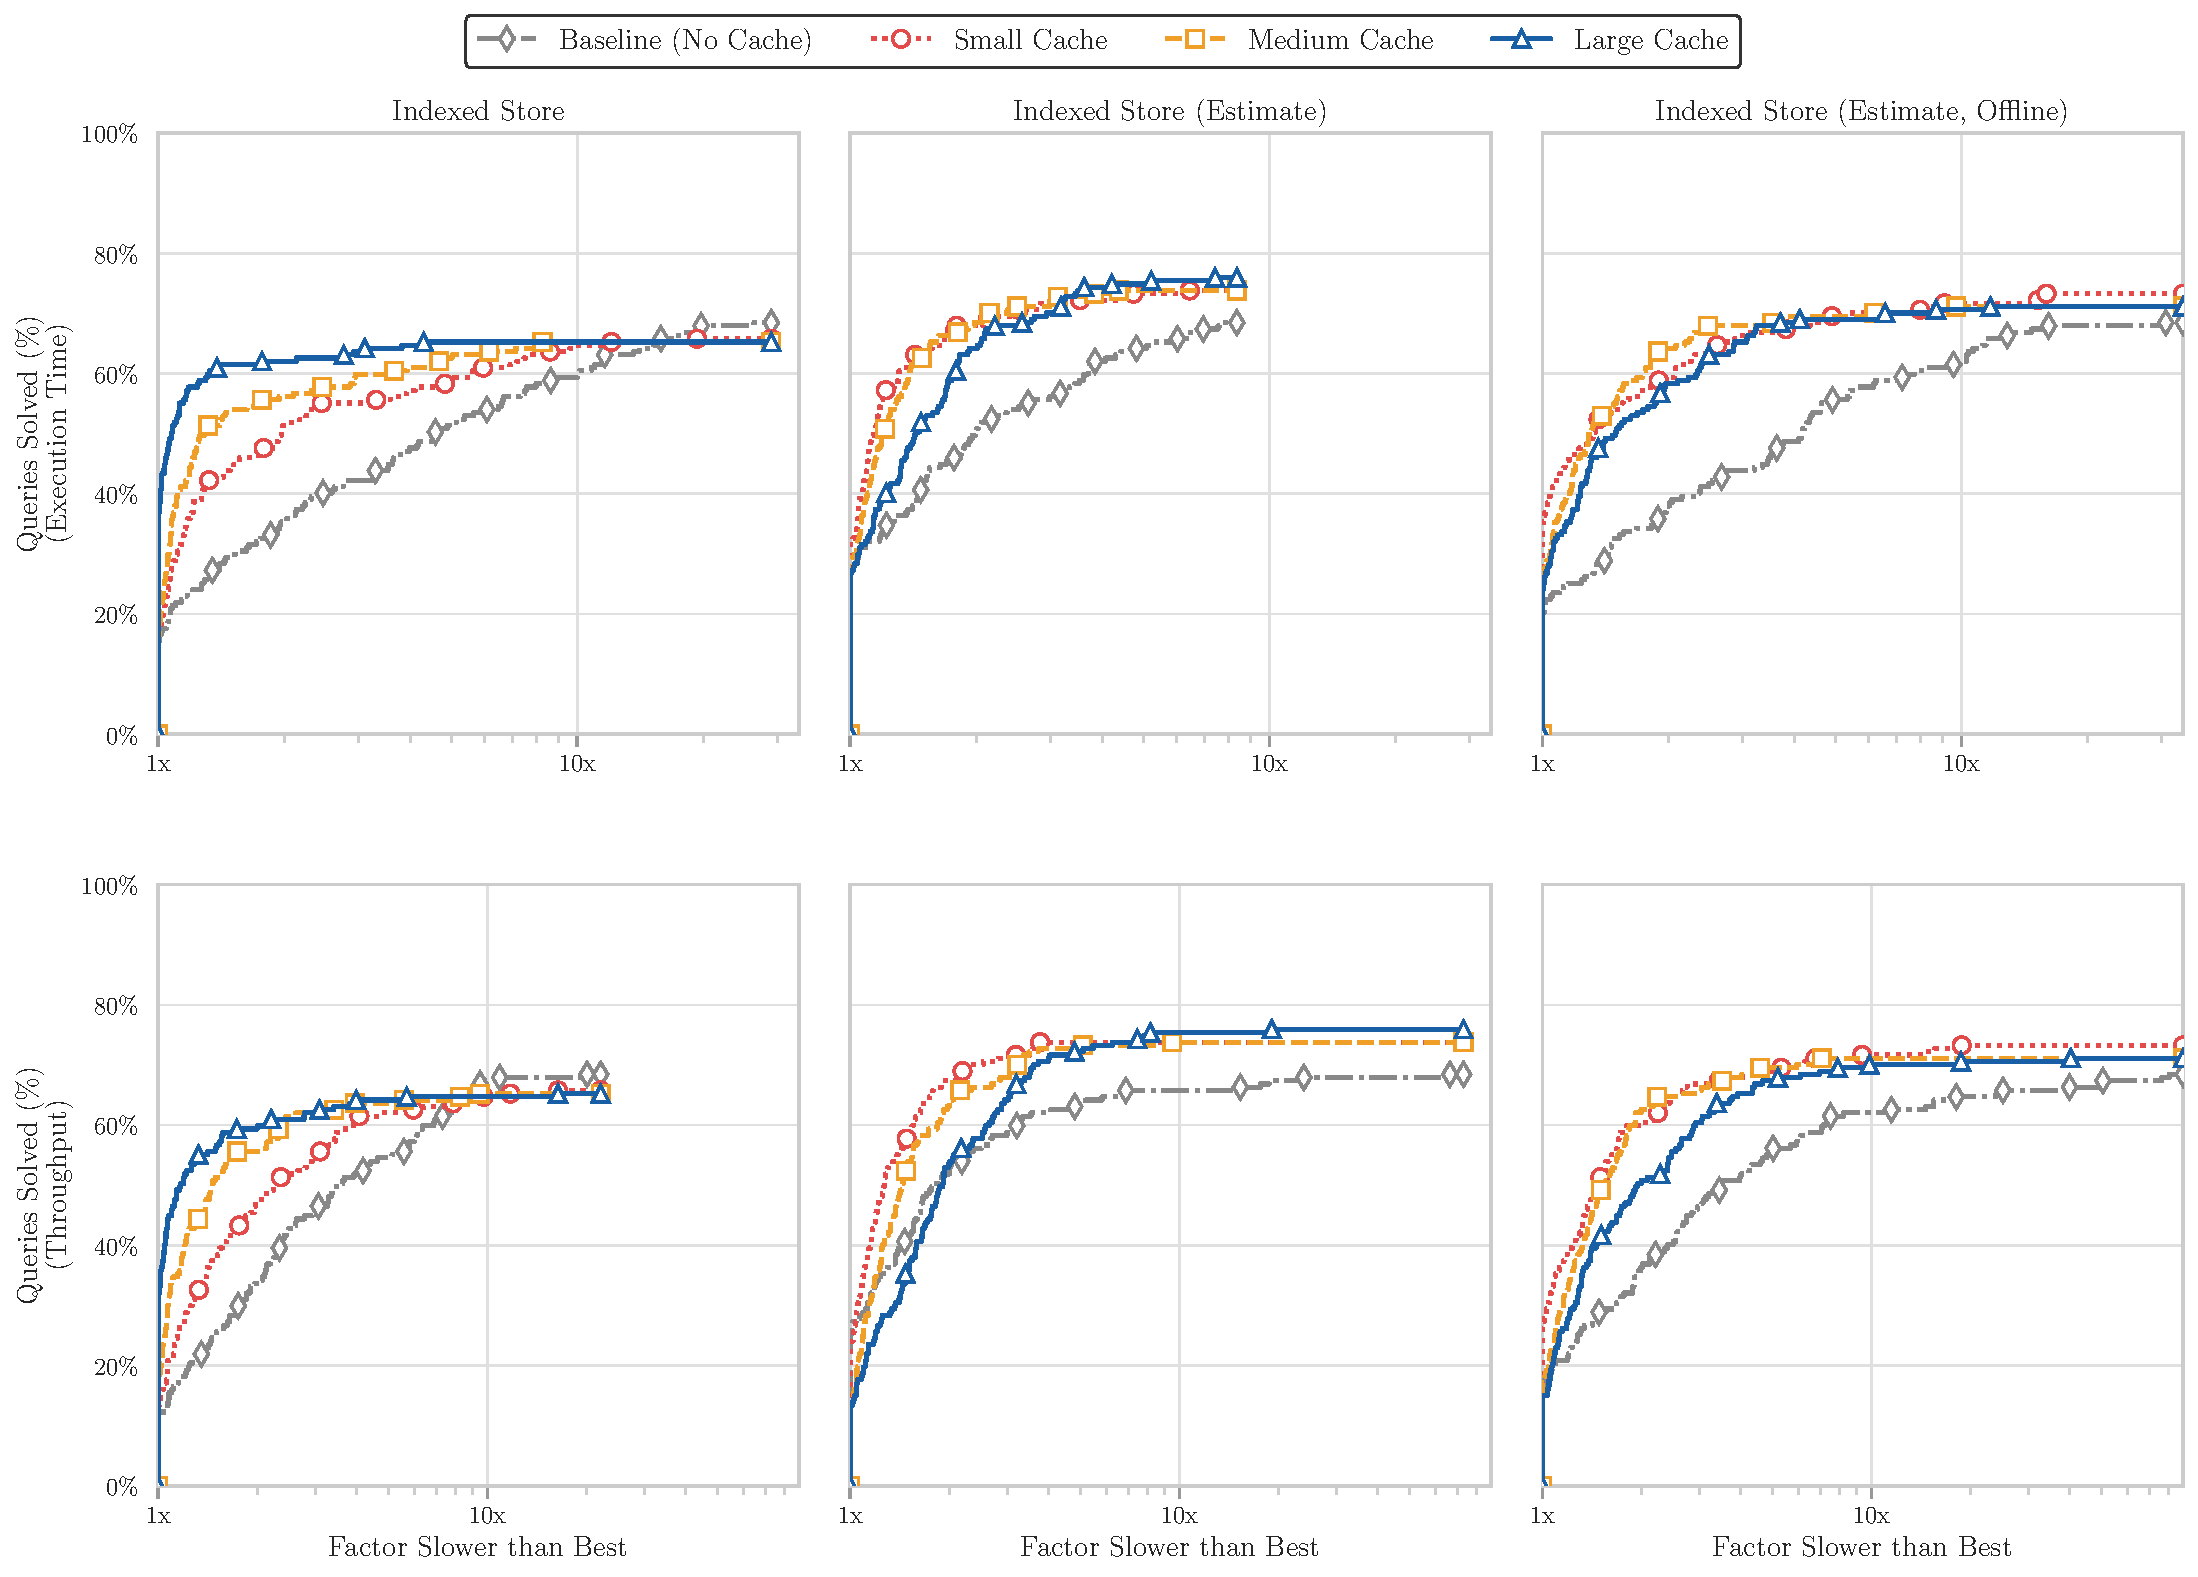
\includegraphics[width=\linewidth]{figures/performance_profile_normal_sequences_store.pdf}
    \caption{Performance profiles of the disk-based quad store cache family of algorithms. 
    The y-axis shows the percentage of queries executing within a factor (x-axis) of the fastest algorithm.
    \todo{PLACEHOLDER FIGURE}}
    \label{fig:disk-store-cache-performance}
\end{figure*}


\paragraph{Comparison Between Caching Algorithms}
\todo{Small section comparing the different caching algorithms and their performance characteristics.
for example how unindex cache mainly improves total execution time, how quad store seems best when
using small caches and LRU-cache scales better for bigger caches.}

\subsubsection{Cache Hitrates}
\todo{Optional section with hitrates and eviction percentages per cache size and algorithm.}


\subsection{Logical Session \& Interest Modeling Cache Performance}

Present a table showing the effect of logical sessions on cache performance. 
Include a metric for the delta number of unique data sources accessed 
during session switches to quantify data locality. 
Discuss the implications of these session dynamics for cache sizing 
and eviction policies.

\subsection{Refinement Patterns}

\todo{Write introduction to this section}

\subsubsection{Effect of chokepoints on query sequences}
\todo{This has a lot of repetition yes?}
We isolated the structural impact of individual query chokepoints through a controlled experiment comprising 80 single-query sequences.
Each sequence begins with a base query and sequentially applies a chain of two to five refinement patterns
from the benchmark's default refinement pattern set.
We repeated each sequence execution 10 times across the three distinct cache capacities (Small, Medium, and Large), 
and measure the cache hit rate, the number of unique data sources accessed, and the total execution time.
For this experiment we only use the LRU-based indexed cache, as we want to analyse the chokepoints 
and their effect on the cache in the simplest configuration.
To quantify the specific performance impact of each chokepoint, 
we mapped the refinement patterns to their underlying chokepoints 
and evaluated them using a linear mixed-effects regression model. 
The model predicts the performance delta ($\Delta Y$) between the current and previous query step. 
We categorize chokepoint operations into two classes: additions (denoted by an `a' suffix) 
and removals (denoted by an `r' suffix). 
A removal operation only occurs when the sequence reverts a previously applied refinement pattern, 
thereby dropping the associated chokepoint from the query. 
The chokepoints added in a given refinement step are represented as a binary vector $X_{t}$, 
where each element indicates the presence (1) or absence (0) of a specific chokepoint. 
These vectors are then used as predictors in the regression model, 
in combination with the previous query's performance metrics ($Y_{t-1}$) to account for the baseline state of the system.
The full regression model is expressed as follows:
\begin{equation}
    \Delta Y_{i,t} = \gamma Y_{i,t-1} + \mathbf{T}_{i,t}^{\top} \boldsymbol{\beta} + u_i + \epsilon_{i,t},
\end{equation}
where $\Delta Y_{i,t}$ is the performance delta for sequence $i$ at refinement step $t$,
$Y_{i,t-1}$ is the previous steps independent variable value, 
$\mathbf{T}_{i,t}$ is a binary indicator vector of the applied chokepoints, 
$\boldsymbol{\beta}$ is the vector of fixed effects estimating the isolated impact of each pattern,
$u_i$ is a sequence-specific random intercept absorbing unobserved heterogeneity across base queries,
and $\epsilon_{i,t}$ is the standard residual error.


Figure~\ref{fig:chokepoint_regression_coefficients} shows the estimated effect of each chokepoint on performance. 
Full regression results are in Appendix~\ref{app:regression_tables} \todo{Verify appendix or supplemental material}.

We observe two types of chokepoint behavior. 
First, modifying some patterns hurts performance in both directions. 
For example, both adding and removing \texttt{T\_3} (increasing required traversal hops) reduces the hit rate and increases execution time.
This reveals a strong cache invalidation penalty: changing the refined query breaks the cache, overwriting much of it and evicting useful data.
From this, we can observe that caching requires a \textit{scan-resistant} algorithm.    

Second, patterns like \texttt{T\_2} (new instantiation values) and \texttt{P\_4} (non-selective triple patterns) have reversible effects. 
Adding these chokepoints drops performance, but removing them improves the hit rate and speeds up execution. 
In these cases, the cache is able to maintain useful data across the refinement, and the chokepoint itself is the primary cause of performance degradation.
Finally, across all patterns, chokepoints that increase the number of accessed data sources consistently lower the cache hit rate.

\paragraph{Implications for Refinement Pattern Design}
From our analysis, we find important weaknesses in our tested caching algorithms. 
We demonstrate that structural mutations like \texttt{T\_3} trigger severe cache invalidation penalties, heavily degrading performance. 
Conversely, the reversible nature of patterns like \texttt{T\_2} proves that caches can successfully maintain temporal locality 
even when the instantiation value, and thus the traversal starting point, changes. 
These findings highlight the importance of our refinement sequence generator and the mapping of refinement patterns to chokepoints.
This mapping allows us to isolate the structural impact of each chokepoint and thus analyse the strengths and weaknesses of a given caching algorithm.
Furthermore, because our sequence generation is dynamically configurable, 
it serves as a targeted diagnostic tool for future systems research. 
Developers can easily extend our default configurations to isolate specific chokepoints, 
allowing them to custom-build stress tests that target the unique operational challenges of their own caching architectures.


The resulting coefficients are given in Figure~\ref{fig:chokepoint_regression_coefficients}, 
where the x-axis represents the estimated effect size of each chokepoint on the performance delta, and the y-axis lists the chokepoints.
For full regression results, we refer to the \todo{Where to put them?}.
From the figure we find that for some chokepoints, such as T.3 (increasing the number of hops required to obtain the data), 
both addition and removal significantly reduce cache hit rate and increase execution time.
Indicating that the chokepoint causes the cache to evict previously cached data, which causes it to underperform when the chokepoint is removed.
Another type of chokepoint, is where the addition of the chokepoint reduces the hitrate and increases execution time, 
while removing it increases hitrate while reducing execution time, such as T.2 (new instantiation value) and P.4 (adding non-selective triple patterns).
Counterintuitively, for chokepoints such as `P.3.r', `P.2.r', and `P.1.a', the large cache has a smaller positive effect 
on hitrate compared to the smaller caches.
As cache hitrate is bound by 1.0, the large cache will have less room for improvement compared to smaller caches, which explains the smaller observed effect.
This is supported by the average hitrates over all queries, which are $0.51$, $0.61$, and $0.66$ for the small, medium, and large caches respectively and the
significant negative coefficient of the lagged cache hitrate value in the regression model, which indicates that a higher previous hitrate reduces the expected change in hitrate.

Finally, we find that in general, chokepoints that significantly increase the number of sources accessed, significantly reduce cache hit rate and vice versa.

\begin{figure*}[htpb]
    \centering
    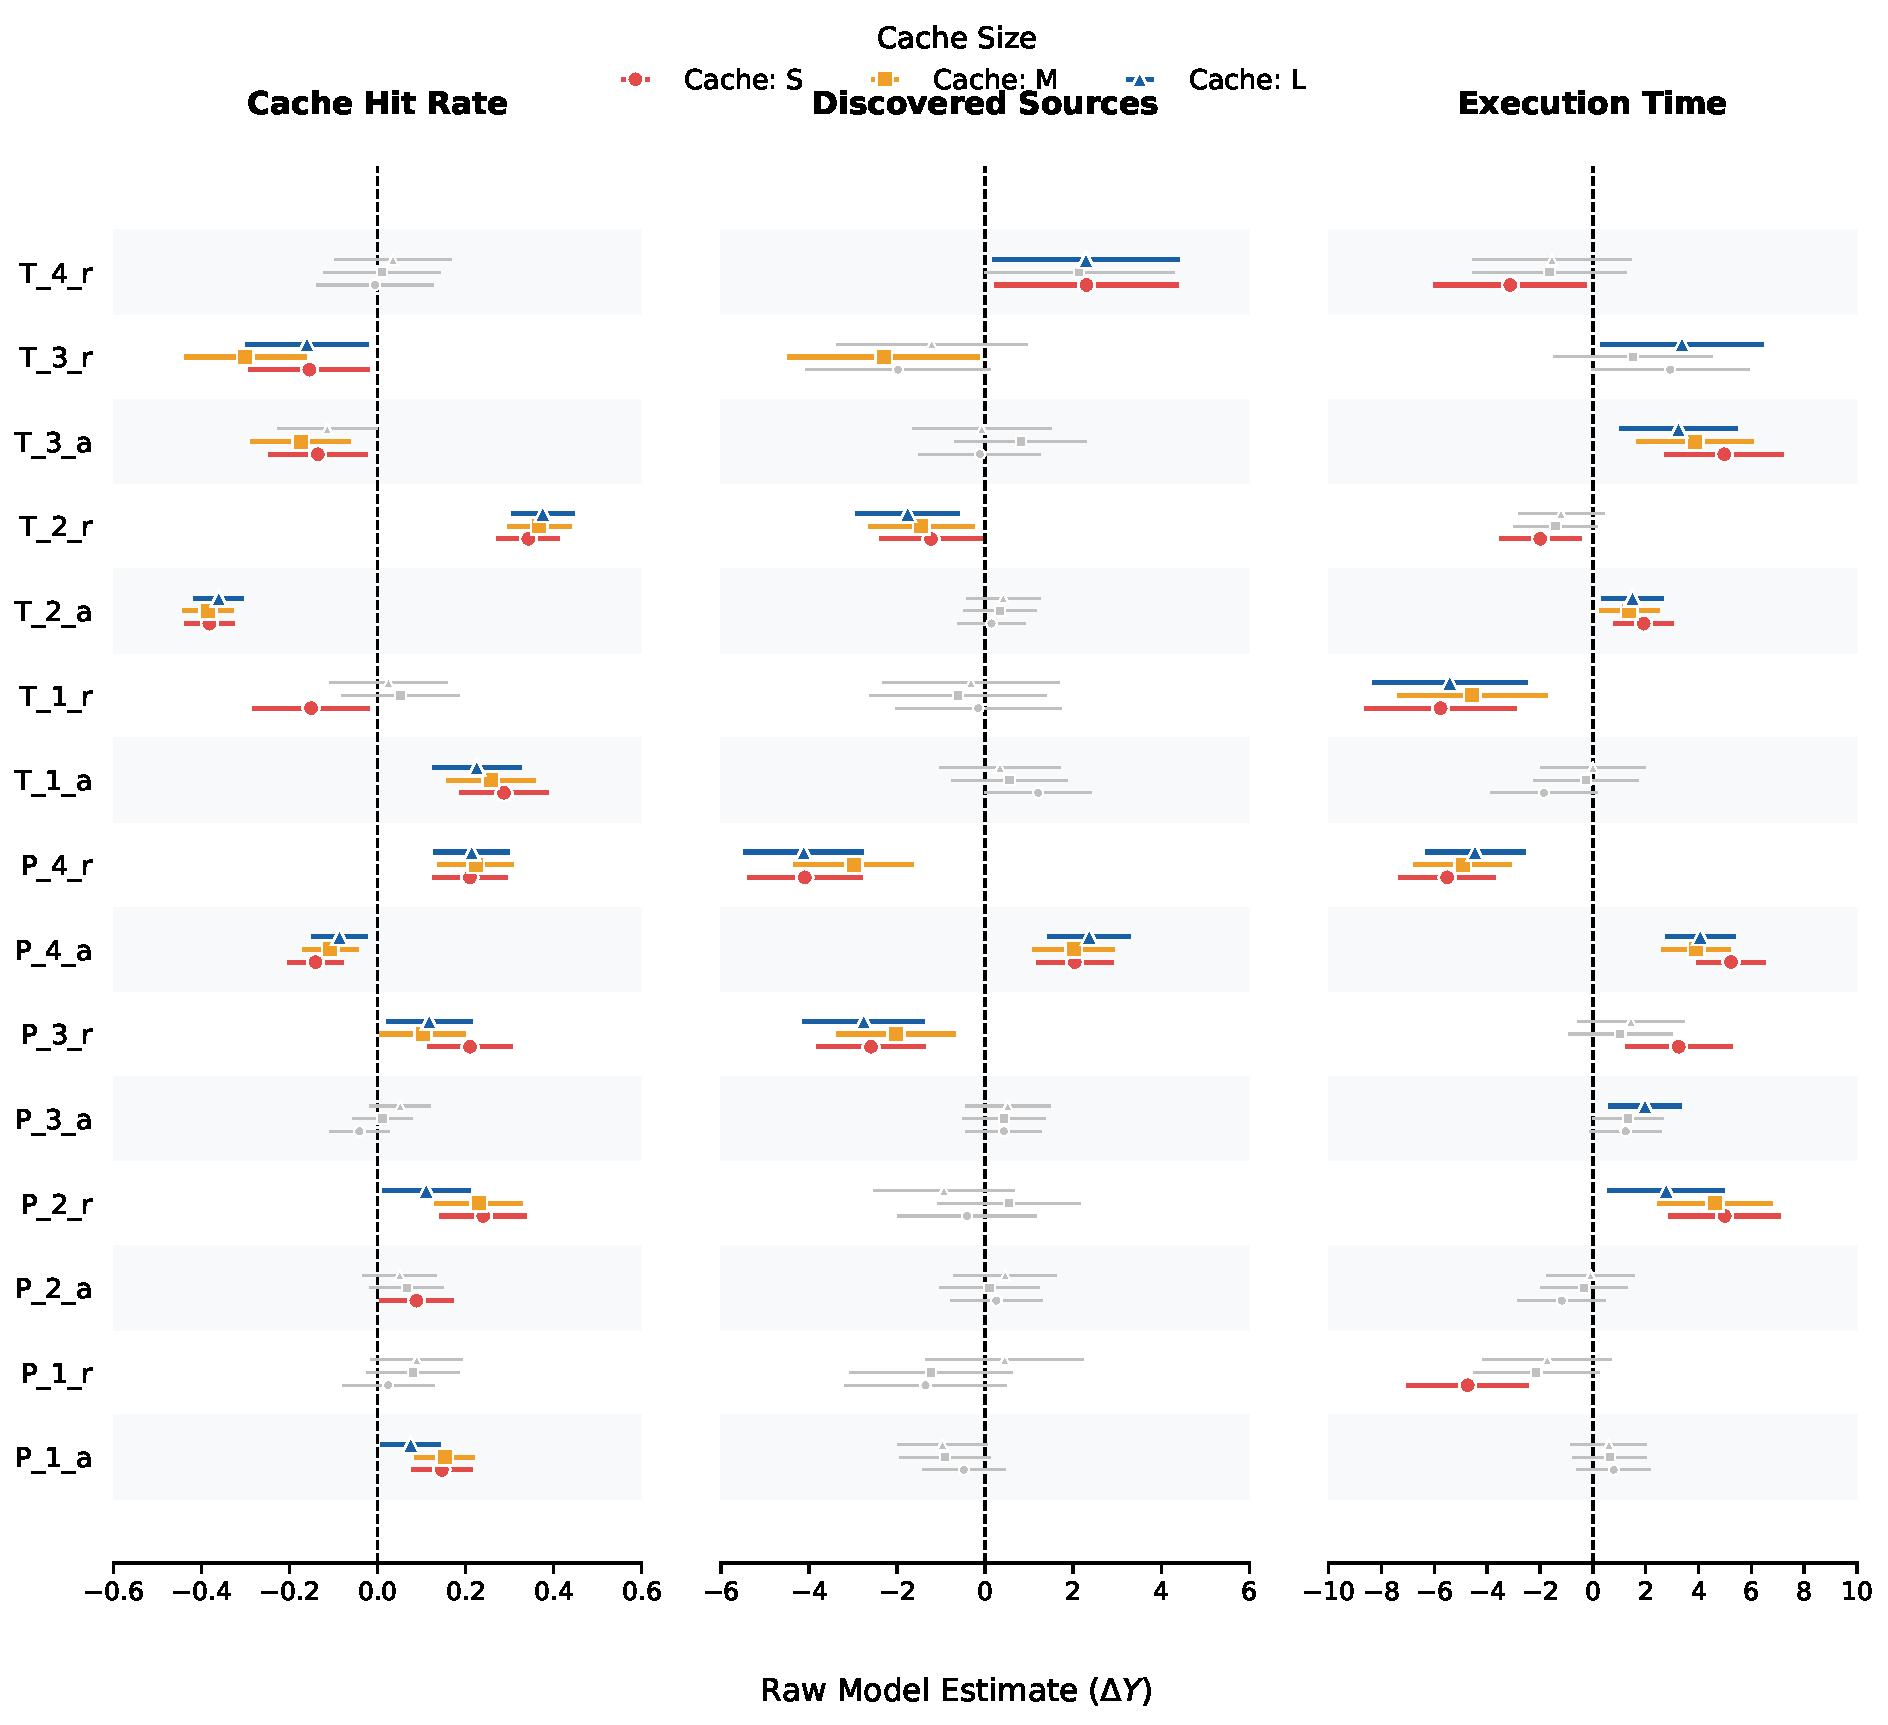
\includegraphics[width=\textwidth]{figures/faceted_forest_figure.pdf}
    \caption{Marginal fixed effects of refinement pattern additions (\texttt{-a}) and removals (\texttt{-r}) on query performance 
        across Small (S), Medium (M), and Large (L) cache capacities. 
        The plot reports the unstandardized absolute expected change ($\Delta Y$) for Cache Hit Rate, Discovered Sources, and Execution Time.
        For both discovered sources and execution time, the plot uses signed log-counts and signed log-milliseconds, respectively.
        Error bars represent $95\%$ confidence intervals and statistically insignificant estimates $(p \ge 0.05)$ are rendered in gray. 
        Undoing the traversal chokepoint changing the instantiation value of the query significantly improves cache hit rate (+.35) and
        reduces the number of unique data sources accessed. However, its effect on execution time is on the edge of significance.}
    \label{fig:chokepoint_regression_coefficients}
\end{figure*}

\subsubsection{Effect of Refinement Depth on Performance}
Next, using default query generation, assess the effect of refinement depth 
on cache performance, followed by implications for cache sizing 
and eviction policies.


\subsection{Comparison to Alternative Evaluation Methods}

The final step in our evaluation is to compare the performance outcomes obtained from our benchmark
against alternative evaluation methods from literature. \todo{Mention random / synthetic}


Compare SolidSessionBench's performance outcomes against alternative 
evaluation methods, specifically micro-benchmarks and random query sequences. 
Highlight differing performance characteristics, identify the analytical 
shortcomings of these alternative methods, explain how their resulting 
conclusions mislead, and demonstrate how this sequence-based benchmark 
resolves those issues.

\paragraph{Microbenchmarks-Theoretical Hit Rate Analysis}
Cache literature extensively uses microbenchmarks of various forms 
to analyze caching performance~\cite{nicholson2024hpcache,hartig2011caching}.
To compare the conclusions of such a benchmark to the conclusions of the benchmark introduced in this paper
we investigate theoretical caching speedup without management costs, 
by executing each query template twice with simulated cache miss probabilities. 
We excluded the estimation-based approaches,
as using the full cache for estimation would skew the results for miss rates above zero.

Figure~\ref{fig:theoretical_cache_performance} shows representative performance profiles for the workload. 
Most templates (8 out of 12) show reliable improvement that scales with the hit rate for both algorithms. 
However, certain long-running queries (e.g., interactive-discover-6, 7, and short-3) show no speedup, 
and some even experience slowdowns. 
These templates traverse many solid pods but do not require all traversed data. 
We hypothesize that rapidly serving documents from an in-memory cache overwhelms the system with data, 
slowing result production. 
Conversely, HTTP network latency gives the JavaScript event loop time to process the join execution pipeline, 
yielding initial results faster since only the first few requests are needed.

In general, using an indexed cache (store-based or LRU) improves performance more than an unindexed cache,
however, this also comes with higher cache management costs, which are not accounted for when using theoretical hit rates.
\todo{See about disk-base caching}
\todo{Circle back to our general evaluation to see how the conclusions differ}

\begin{figure*}[!h]
    \centering
    % Ensure the filename matches your generated PDF
    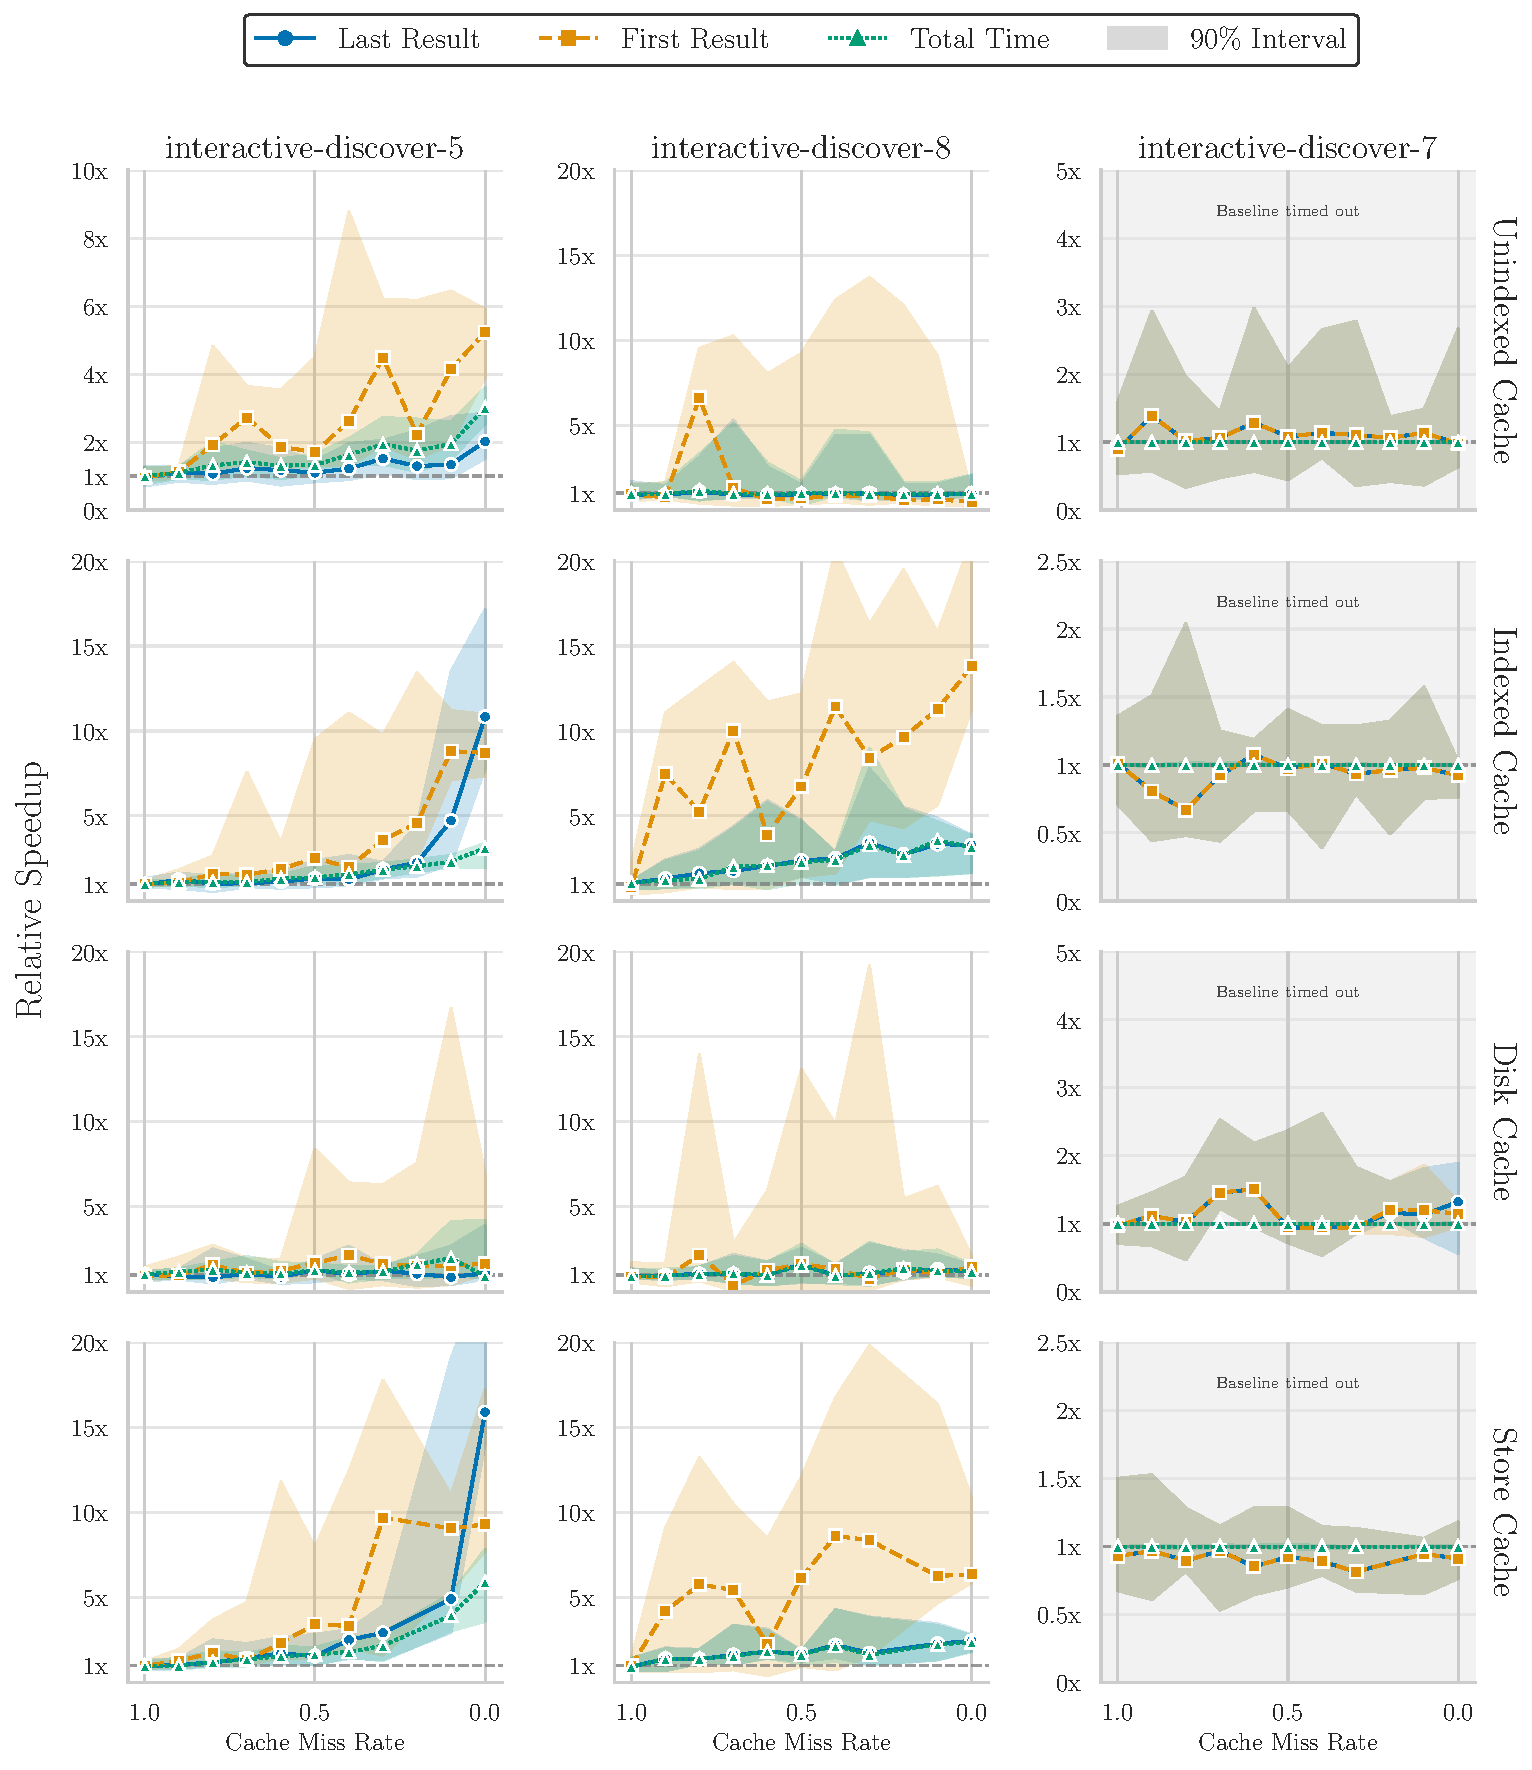
\includegraphics[width=\textwidth]{figures/synth_hit_rate_reduced_combined.pdf}
    \caption{ Performance of unindexed, LRU indexed, In-memory store, and Disk-based store caches 
    across representative query templates. The y-axis shows the mean speedup relative 
    to a baseline with a 0\% hit rate. Shaded regions denote the 90th percentile
    \todo{Placeholder disk figure}}
    \label{fig:theoretical_cache_performance}
\end{figure*}

\paragraph{Random Query Sequences}



\paragraph{Scope and Limitations}
We evaluate SolidSessionBench against microbenchmarks and random sequences, 
but explicitly exclude hand-crafted scenarios and simple distributions.
Hand-crafted methods lack scalability, while simple distributions fail to capture complex user habits.
By automating logical sessions and user interests, our benchmark functions as a scalable superset of both approaches,
making direct comparison redundant. 
By contrast, the compared methods do not incorporate these sequence attributes, 
and our results show this omission risks drawing inaccurate conclusions.

% We evaluate our benchmark using a scale 0.1 SolidBench dataset comprising 158,233 RDF files,
% 1,531 vaults, and 3,556,159 triples. 
% Applying the default hyperparameters from Table~\ref{tab:generation_hyperparameters},
% we generated 8 sequences totaling 192 interactive-workload queries, encompassing both discover and short templates.
% Experiments were conducted on an Ubuntu 20.04 machine (Intel Core i5-9400) with 16 GB RAM and a 180-second timeout.
% To minimize variance and simulate realistic networks, we repeated each sequence 10 times with 70–90 ms injected latency 
% to simulate realistic network conditions.
% Caches were scoped to individual sequences, ensuring no state was shared between repetitions. 

% These experiments aim to test our sequence generation by assessing how our design choices influence 
% query correlation, measured via cache hit rates and evictions, 
% and to establish a caching performance baseline for a Link Traversal-based Query Processing (LTQP) engine.
% While we report speedups to demonstrate utility, the primary focus is benchmark validation rather than exhaustive algorithm evaluation.  


% We evaluate our benchmark using a scale 0.1 SolidBench dataset 
% (158,233 RDF files, 1,531 vaults, 3,556,159 triples). 
% Using the default hyperparameters in Table~\ref{tab:generation_hyperparameters}, 
% we generate 8 sequences totaling 192 queries. 
% These queries are from the interactive workload, are split into discover and short queries,
% with multiple templates belonging to either of these groups.
% Experiments run on an Ubuntu 20.04 machine (Intel Core i5-9400) 
% with 16 GB RAM allocated to the engine and a 180-second query timeout. 
% We repeat each sequence 10 times to minimize variance and 
% inject a uniform 70–90 ms latency to simulate a realistic network environment.
% The cache is scoped for a sequence, meaning no cache-state is shared between different executions or repetitions of
% sequences.

% These experiments serve two goals. 
% Primarily, we validate the sequence generation by assessing how our three 
% design choices impact query correlation, measured via cache \textit{hit rates} and \textit{evictions}. 
% Secondarily, we establish a caching performance baseline for a LTQP engine. 
% While we report execution speedups to demonstrate the benchmark's utility, 
% our focus is on validating the benchmark design rather than exhaustively evaluating the caching algorithms.

% \rt{Can you briefly hint to the subsections that will come hereafter? (so the reader knows what to expect)}

% \subsection{Global Cache Performance}

% Figure~\ref{fig:global_cache_performance} compares performance profiles~\cite{dolan2002benchmarking} 
% for each approach against the no-cache baseline. 
% As expected, all caching methods outperform the baseline.

% \begin{figure*}[t]
%     \centering
%     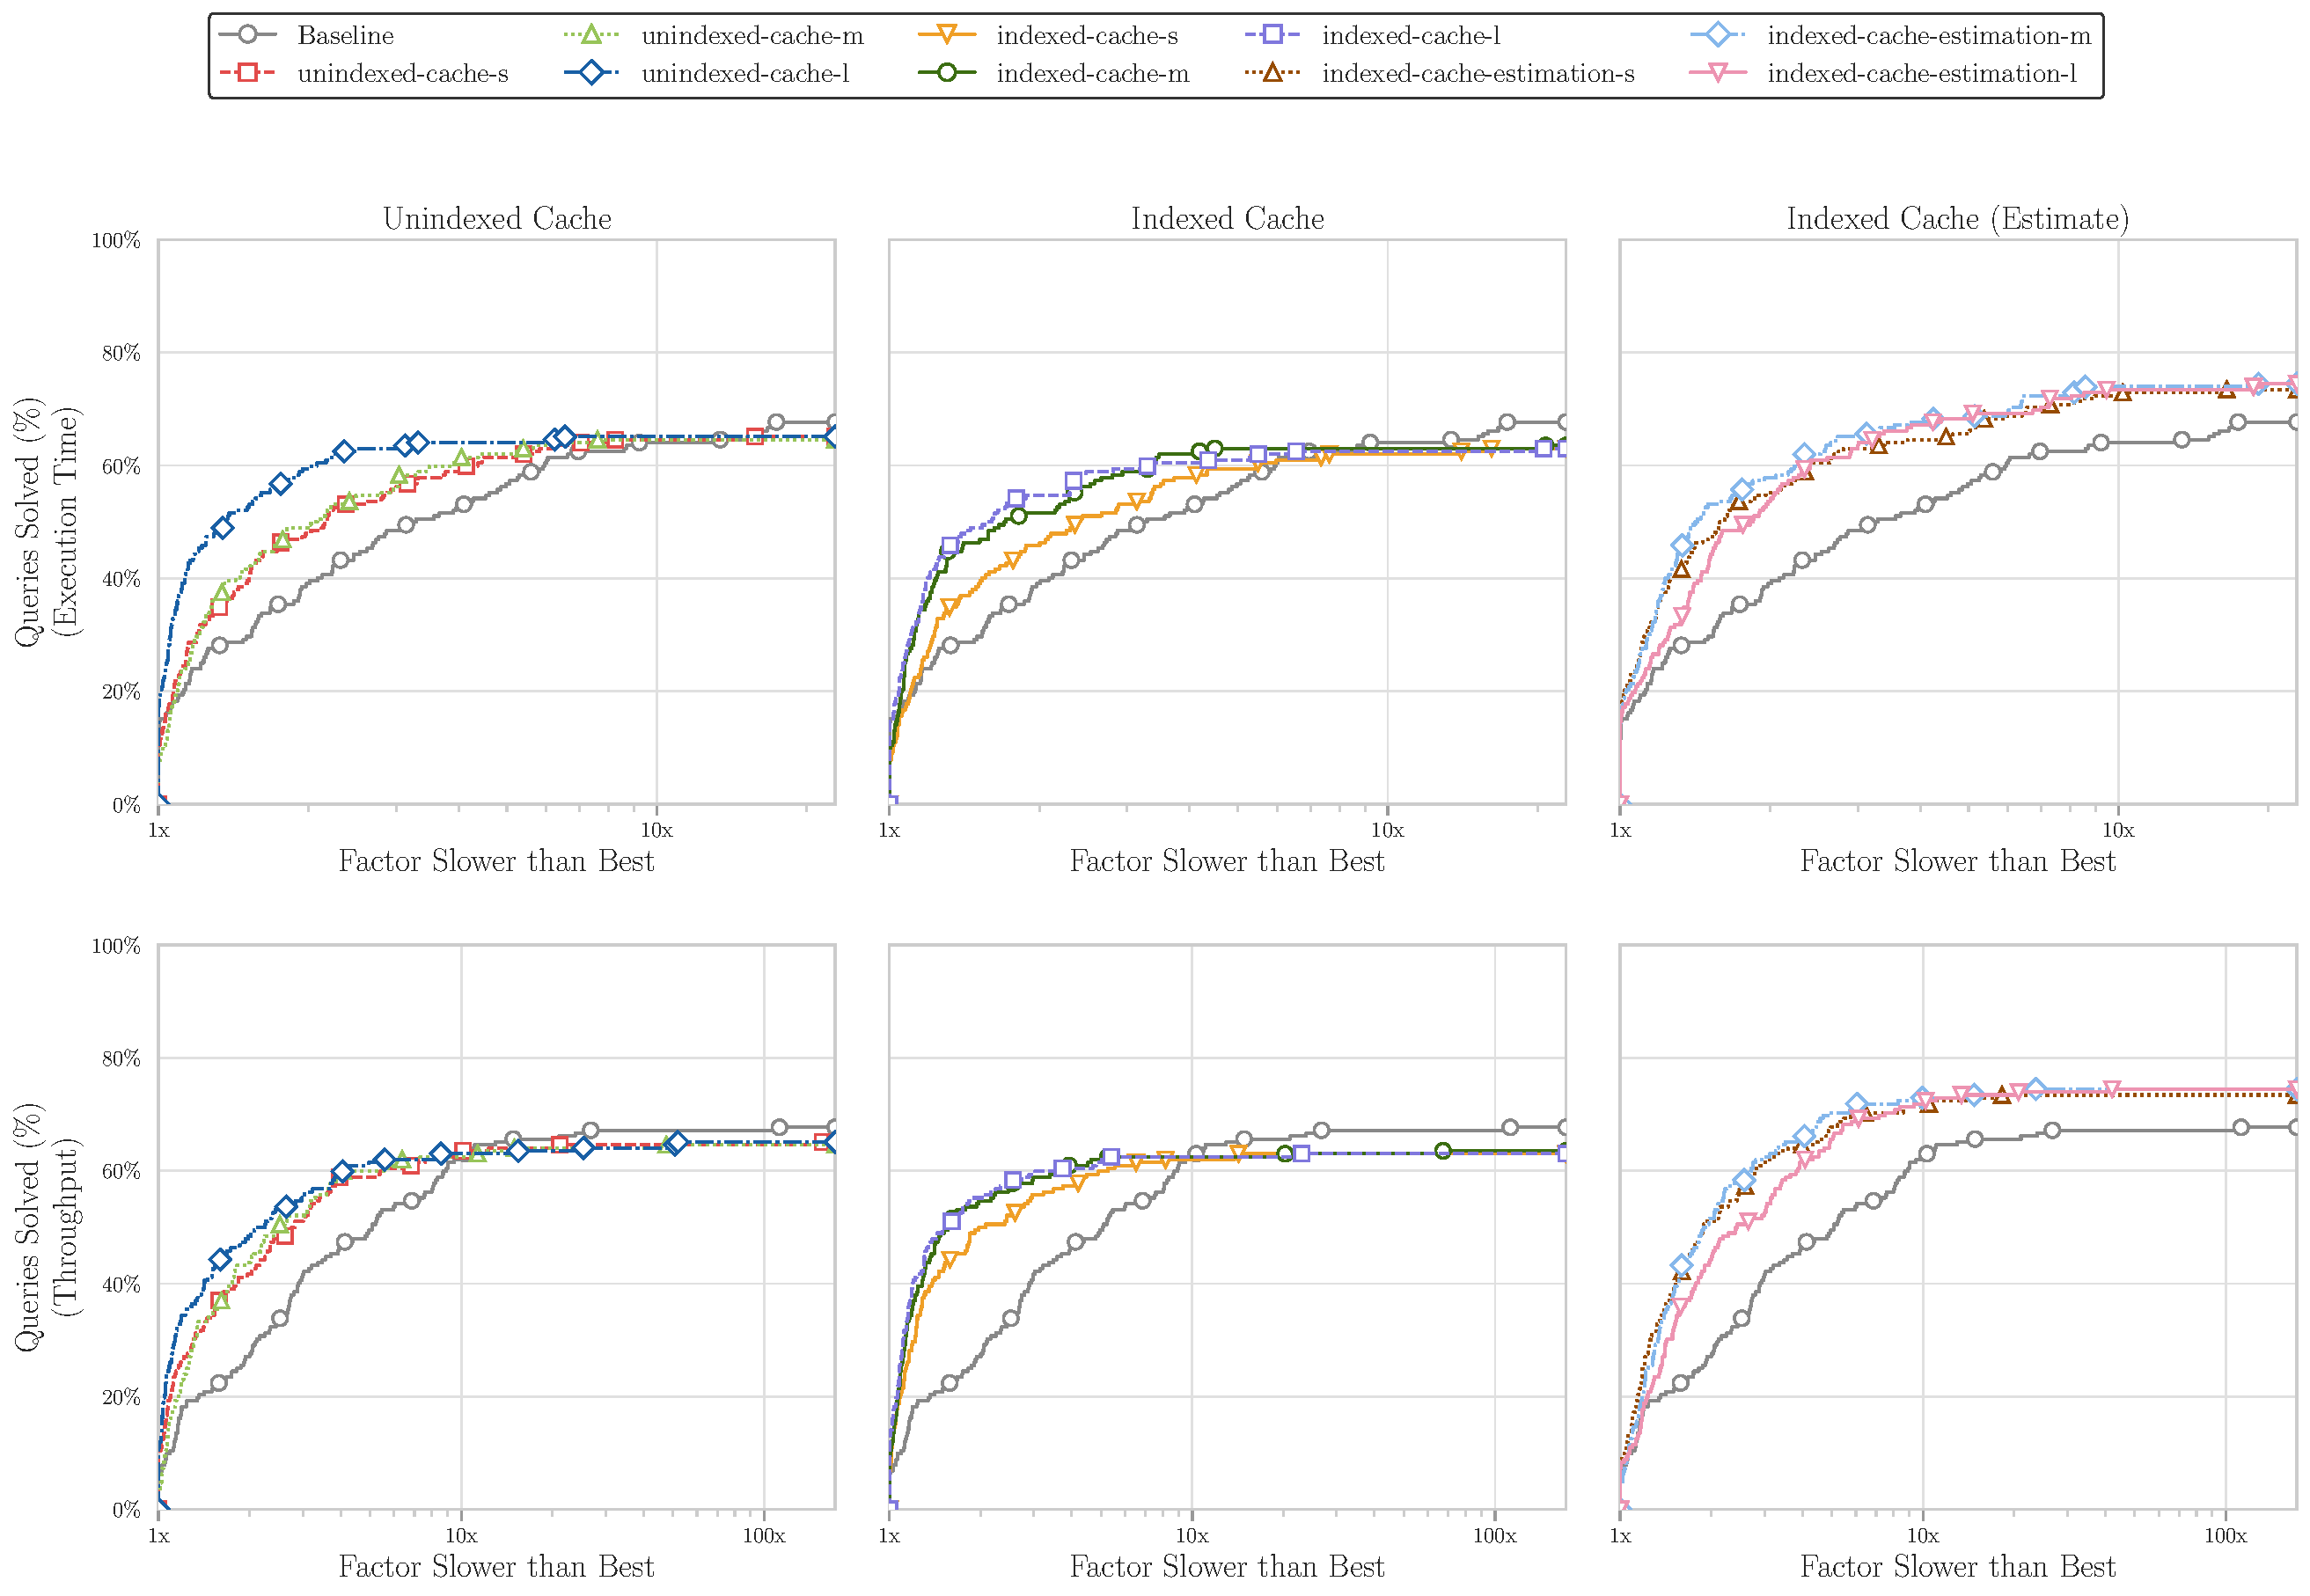
\includegraphics[width=\linewidth]{figures/performance_profile.pdf}
%     \caption{Performance profiles of the tested cache algorithms. 
%     The y-axis shows the percentage of queries executing within a factor (x-axis) of the fastest algorithm. 
%     Curves closer to the top-left indicate better overall performance. 
%     The y-intercept ($x=1$) shows how often an algorithm is the outright fastest, 
%     while the rightward trajectory demonstrates robustness 
%     (e.g., $x=2, y=80\%$ means 80\% of queries execute within twice the fastest time).
%     From the figure, we observe that all caching-based approaches outperform the no-cache baseline.}
%     \label{fig:global_cache_performance}
% \end{figure*}


% For the unindexed cache, 
% small (350k triples) and medium (700k triples) sizes perform similarly. 
% The large cache (1,400k triples) significantly improves speed by retaining enough entries across the sequence.
% However, the baseline resolves more total queries, 
% suggesting cache management overhead causes timeouts for longer queries.

% The indexed cache has a higher failure rate, 
% as initial indexing costs slow execution when the eviction rate outweighs the increased efficiency of cache hits. 
% Still, it accelerates successful queries more than the unindexed cache. 
% It also reaches critical capacity sooner, with medium and large sizes performing similarly.

% Overall, the indexed cache with cardinality estimation performs best, 
% increasing speed and solving more queries. 
% Notably, larger cache sizes degrade performance. 
% A possible mechanism for this is that the estimator evaluates all cache entries,
% including irrelevant unreachable data from past queries. 
% This accumulated noise likely can degrade estimates, suggesting the estimator favors smaller, fresher caches.

% \subsection{Logical Sessions}
% To evaluate the impact of logical sessions on caching performance, 
% we analyze the hit rate deviation ($\Delta$) from the overall average when queries initiate a new session, 
% switch to an existing one, or remain in the current session.
% Table~\ref{tab:performance_differences} shows that new sessions severely degrade hit rates,
% existing session switches cause moderate degradation, and intra-session queries improve performance.
% These effects are strongest in small and medium caches.

% Consequently, optimal client-side cache sizing depends heavily on user session-switching behavior.
% These findings highlight the need for eviction policies that better retain cross-session entries
% and validate our simulation design;
% ignoring session dynamics would obscure critical real-world performance shifts.

% Future work should investigate whether query sequences should share a frequently accessed core of cache entries.
% Protecting these entries from eviction could mitigate the performance penalties of session switching.
% Engines could also attempt to identify sessions and keep seperate caches for each session.

% \begin{table*}[htpb]
% \centering
% \caption{
%     Impact of logical session status on algorithm performance. 
%     Values represent absolute and percentage cache hit rate deviations from the global template average across 
%     new, existing, and within-session queries. Negative values mean caches perform worse for these types of
%     queries.
% }
% \label{tab:performance_differences}
% \begin{tabular*}{\textwidth}{@{\extracolsep{\fill}} l r@{\hspace{1em}}r r@{\hspace{1em}}r r@{\hspace{1em}}r @{}}
% \toprule
% \textbf{Cache Algorithm} & \multicolumn{2}{c}{\textbf{New Session}} & \multicolumn{2}{c}{\textbf{Existing Session}} & \multicolumn{2}{c}{\textbf{Within Session}} \\
% \cmidrule(lr){2-3} \cmidrule(lr){4-5} \cmidrule(lr){6-7}
% & \textbf{Abs.} & \textbf{\%} & \textbf{Abs.} & \textbf{\%} & \textbf{Abs.} & \textbf{\%} \\
% \midrule
% unindexed-l        & -0.066 & -12.278 & -0.014 & -2.474 &  0.011 &  1.931 \\
% unindexed-m        & -0.056 & -15.649 & -0.031 & -7.900 &  0.024 &  5.486 \\
% unindexed-s        & -0.071 & -24.275 & -0.021 & -6.551 &  0.017 &  4.582 \\
% \cmidrule(lr){1-7}
% indexed-estimate-l & -0.053 & -10.573 & -0.015 & -2.796 &  0.012 &  2.127 \\
% indexed-estimate-m &  0.028 &   7.174 & -0.000 & -0.064 & -0.000 & -0.035 \\
% indexed-estimate-s & -0.044 & -14.305 & -0.013 & -3.921 &  0.010 &  2.924 \\
% \cmidrule(lr){1-7}
% indexed-l          & -0.026 &  -5.011 & -0.003 & -0.571 &  0.003 &  0.467 \\
% indexed-m          & -0.087 & -22.782 & -0.021 & -5.098 &  0.017 &  3.682 \\
% indexed-s          & -0.033 & -11.036 & -0.015 & -4.470 &  0.012 &  3.153 \\
% \bottomrule
% \end{tabular*}
% \end{table*}

% \subsection{Refinement Patterns}

% To evaluate iterative query refinement simulation, 
% we analyze cache behavior across refinement depths. 
% Figure \ref{fig:cache_efficiency} shows that hit ratios increase progressively 
% as queries undergo sequential refinement. 
% Across all algorithms, hit rates increase at depths 2 and 3, 
% confirming that refinement heavily reuses prior data.

% \begin{figure*}[htpb]
%     \centering
%     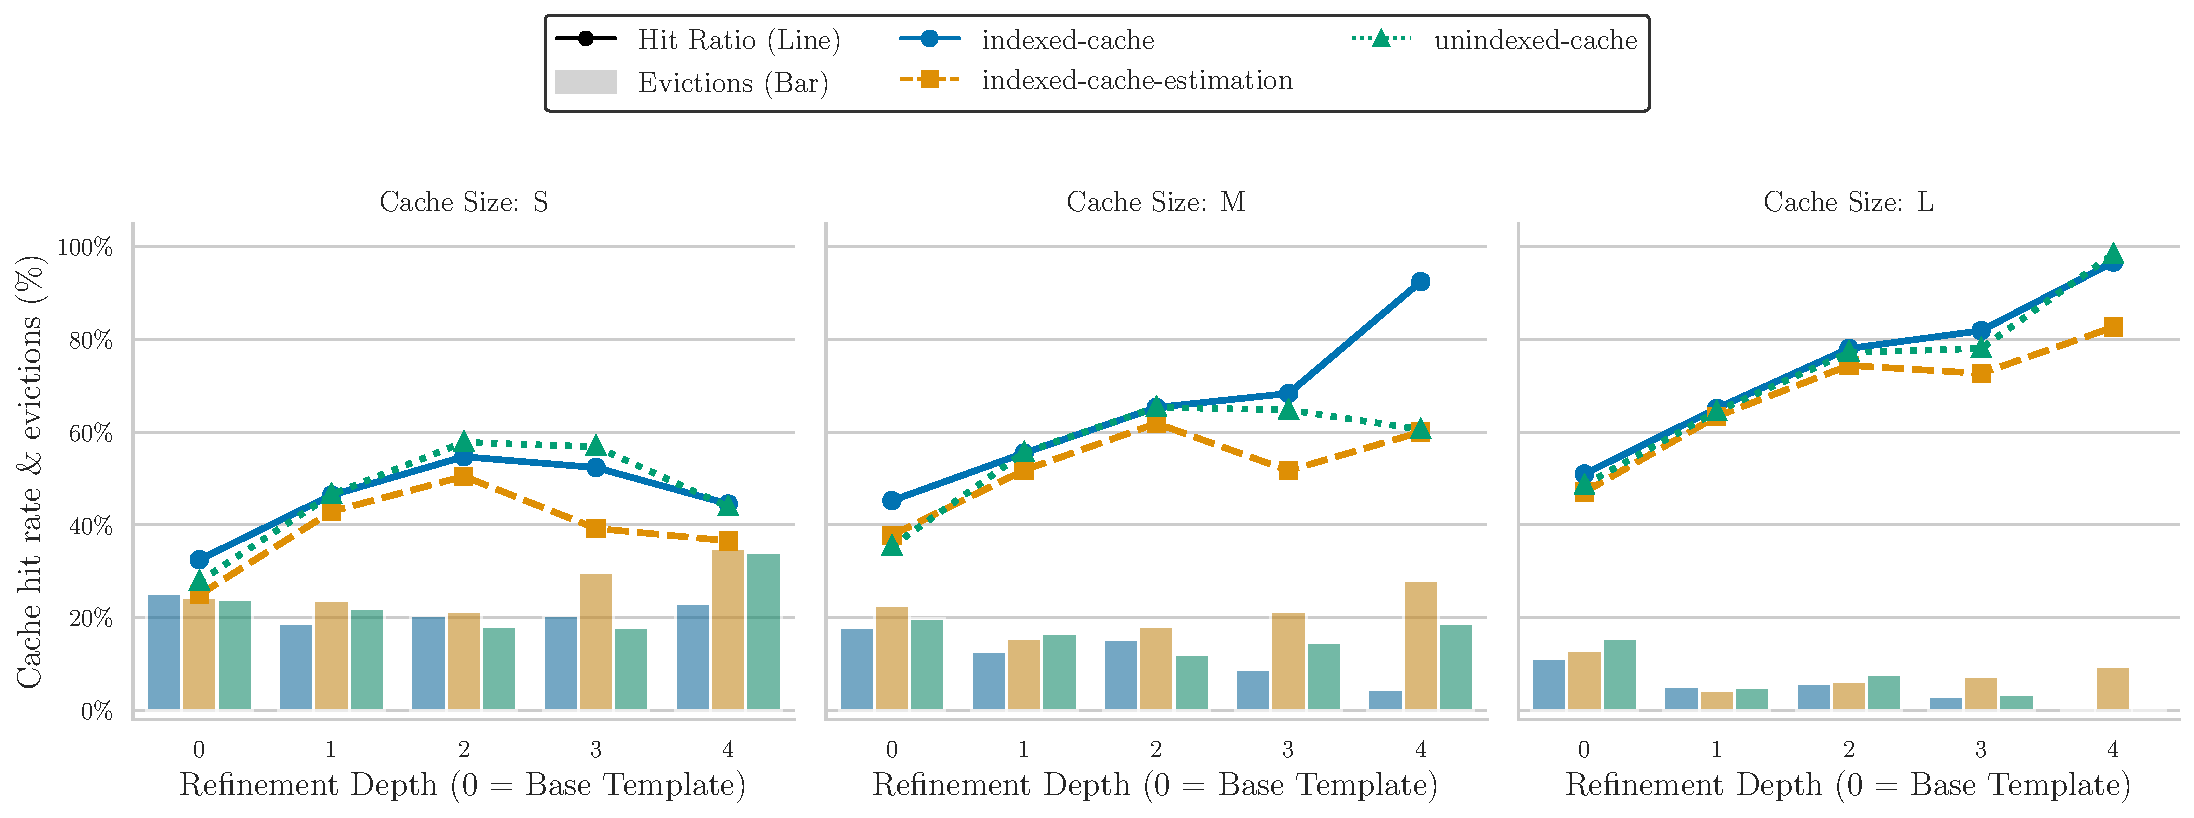
\includegraphics[width=\textwidth]{figures/combined_cache_efficiency.pdf}
%     \caption{Cache hit ratios and percentage of cache capacity evicted across refinement depths for small, medium, and large cache configurations.}
%     \label{fig:cache_efficiency}
% \end{figure*}

% At higher refinement depths, 
% performance depends heavily on cache capacity. 
% Large caches sustain high hit rates through depth 4, 
% whereas small caches experience significant thrashing,
% and degraded hit ratios. 

% Surprisingly, the indexed cache without estimation maintains high hit rates at small capacities. 
% Different caching mechanisms alter how the Node.js event loop schedules traversal and join executions,
% changing traversal order and rate.
% We suspect this variance increases temporal locality, though further analysis is needed to confirm the exact mechanism and explain why the indexed cache outperforms the unindexed baseline.

% The observed cache hit rate and eviction differences directly translate to measurable execution speedups.
% Figure 2 illustrates that the geometric mean speedup generally scales positively with refinement depth, with 
% a more pronounced effect for the throughput. 
% The indexed-cache algorithm proves particularly effective for prolonged exploratory sequences,
% achieving substantial throughput gains at depth 4 compared to the unindexed alternatives.

% \begin{figure*}[htpb]
%     \centering
%     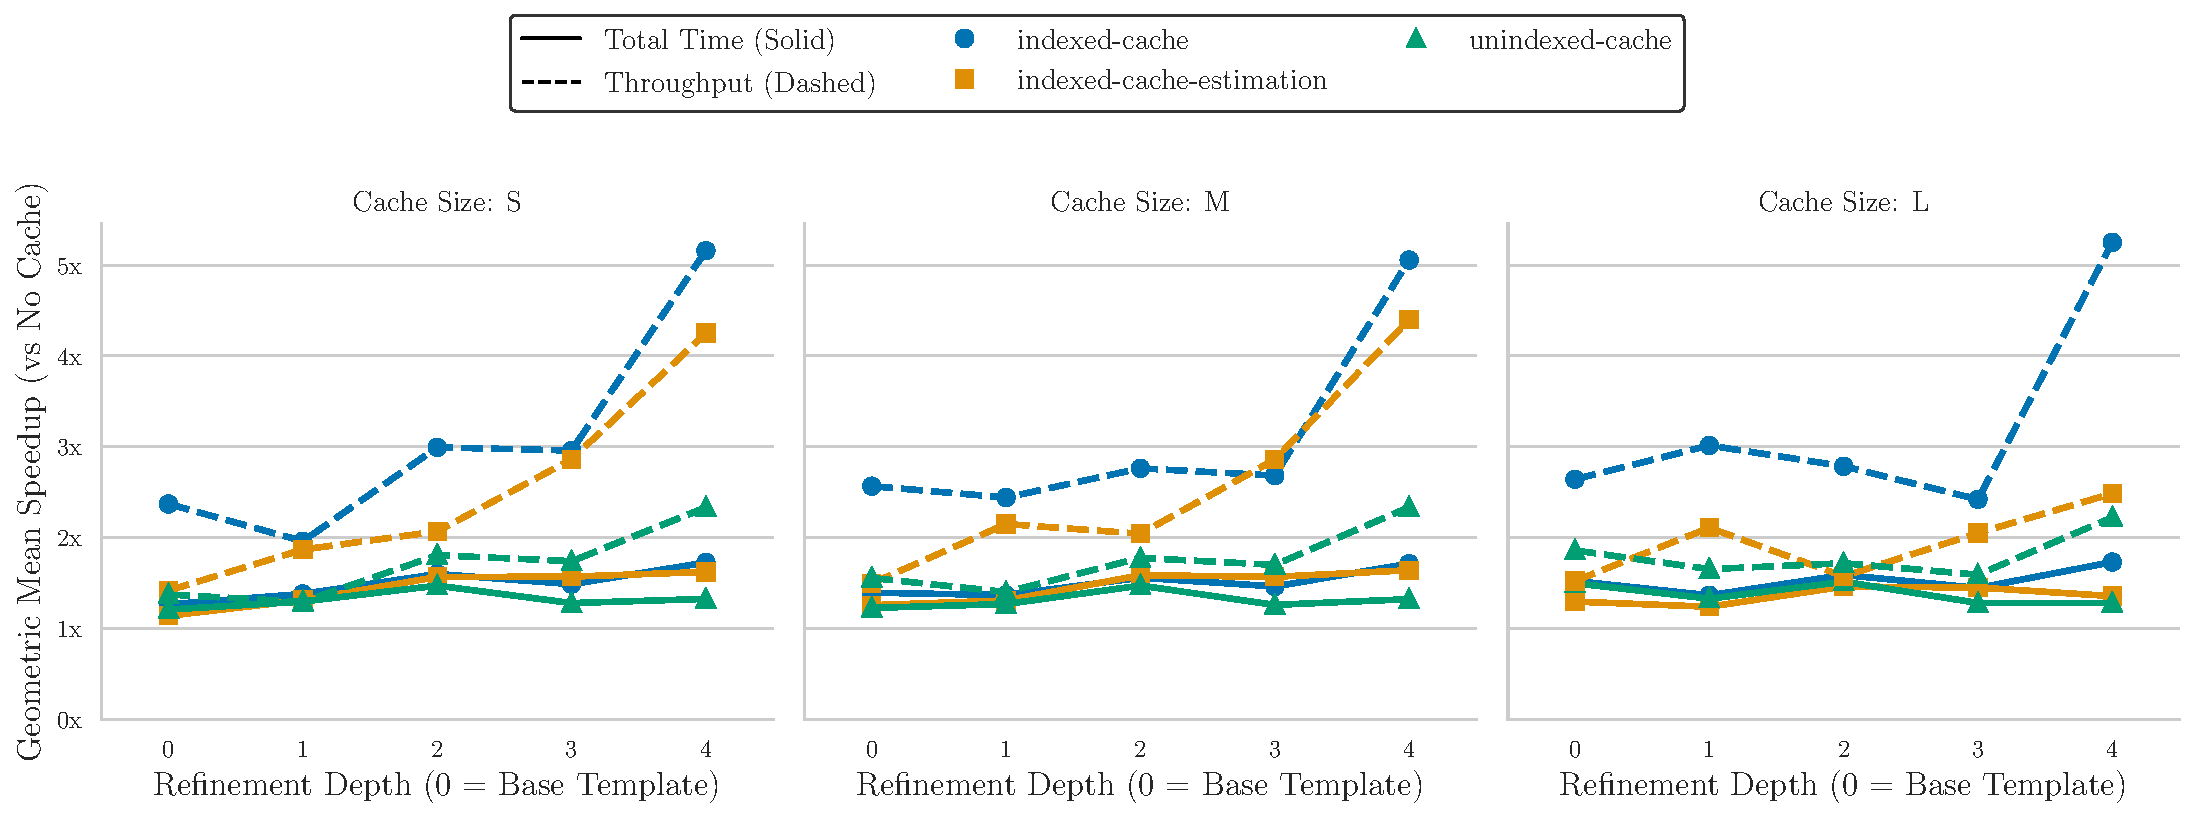
\includegraphics[width=\textwidth]{figures/temporal_throughput_line.pdf}
%     \caption{Geometric mean of observed speedups and increases respectively for total execution time and query throughput 
%     relative to the no caching baseline across refinement depths.}
%     \label{fig:temporal_throughput}
% \end{figure*}

% \subsection{Comparison To Other Evaluation Methods}

% \paragraph{Microbenchmarks-Theoretical Hit Rate Analysis}

% Cache literature extensively uses microbenchmarks of various forms 
% to analyze caching performance~\cite{nicholson2024hpcache,hartig2011caching}.
% To compare the conclusions of such a benchmark to the conclusions of the benchmark introduced in this paper
% we investigate theoretical caching speedup without management costs, 
% by executing each query template twice with simulated cache miss probabilities. 
% We excluded the estimation-based approach, 
% as using the full cache for estimation would skew the results for miss rates above zero.

% Figure~\ref{fig:theoretical_cache_performance} shows representative performance profiles for the workload. 
% Most templates (8 out of 12) show reliable improvement that scales with the hit rate for both algorithms. 
% However, certain long-running queries (e.g., interactive-discover-6, 7, and short-3) show no speedup, 
% and some even experience slowdowns. 
% These templates traverse many solid pods but do not require all traversed data. 
% We hypothesize that rapidly serving documents from an in-memory cache overwhelms the system with data, 
% slowing result production. 
% Conversely, HTTP network latency gives the JavaScript event loop time to process the join execution pipeline, 
% yielding initial results faster since only the first few requests are needed.

% \begin{figure*}[!h]
%     \centering
%     % Ensure the filename matches your generated PDF
%     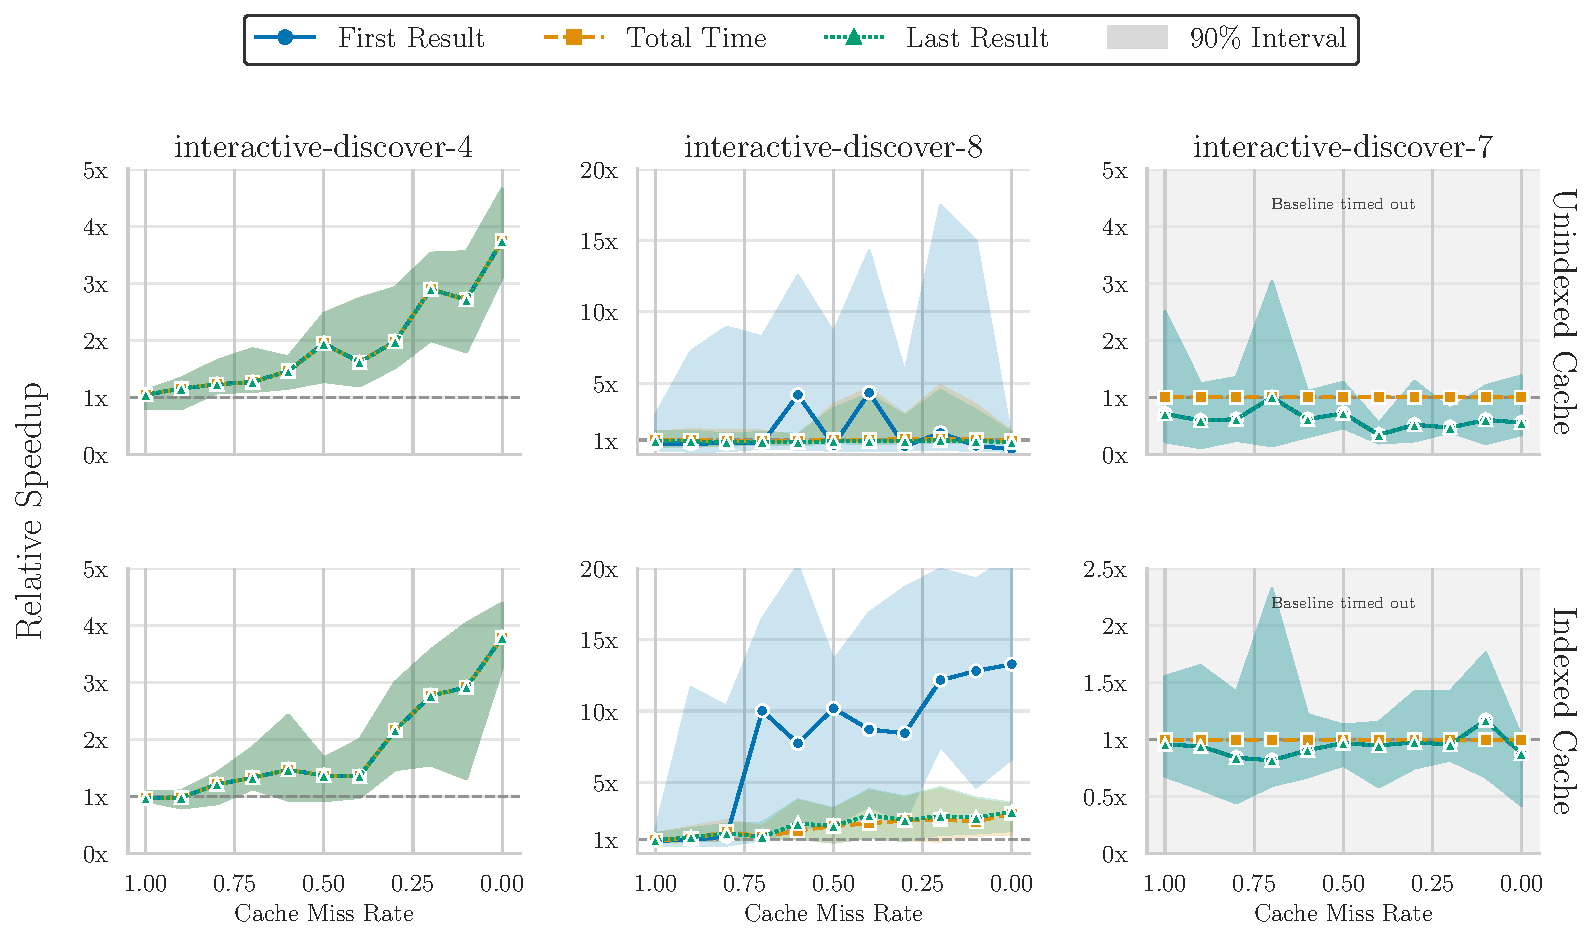
\includegraphics[width=\textwidth]{figures/synth_hit_rate_reduced.pdf}
%     \caption{ Performance of unindexed and indexed caches across representative query templates. 
%     The y-axis shows the mean speedup relative to a baseline with a 0\% hit rate.
%      Shaded regions denote the 90th percentile}
%     \label{fig:theoretical_cache_performance}
% \end{figure*}

% Both caching approaches perform similarly overall, 
% but the indexed cache significantly reduces time-to-first-result across most templates. 
% As expected, indexed caching is highly advantageous without evictions. 
% However, the initial indexing cost creates a trade-off: 
% it amplifies both speedups and slowdowns relative to an unindexed cache. 
% While this micro-benchmark approach aligns with prior literature~\cite{nicholson2024hpcache}, 
% our mixed findings show that micro-benchmarks alone fail to thoroughly evaluate client-side caching optimizations. 
% This limitation demonstrates the clear need for the comprehensive benchmark we introduce in this work.




% \paragraph{Random Query Sequences}
% Another common approach is to use random query sequences from an existing 
% benchmark~\cite{o2009star,bizer2011berlin,hartig2011caching,nicholson2024hpcache,folz2016cyclades}.
% Figure~\ref{fig:global_cache_performance_random_sequences} shows execution times 
% for sequences created by randomly grouping default SolidBench.js queries.
% For these random sequences, only large caches perform well,
% while smaller ones degrade below the baseline.
% These results misleadingly suggest that large caches are vital, 
% whereas our benchmark demonstrates significant performance benefits even with smaller sizes.
% As expected, the estimation cache performs well in both scenarios because cardinality estimation does not require cache hits.

% \begin{figure*}[htpb]
%     \centering
%     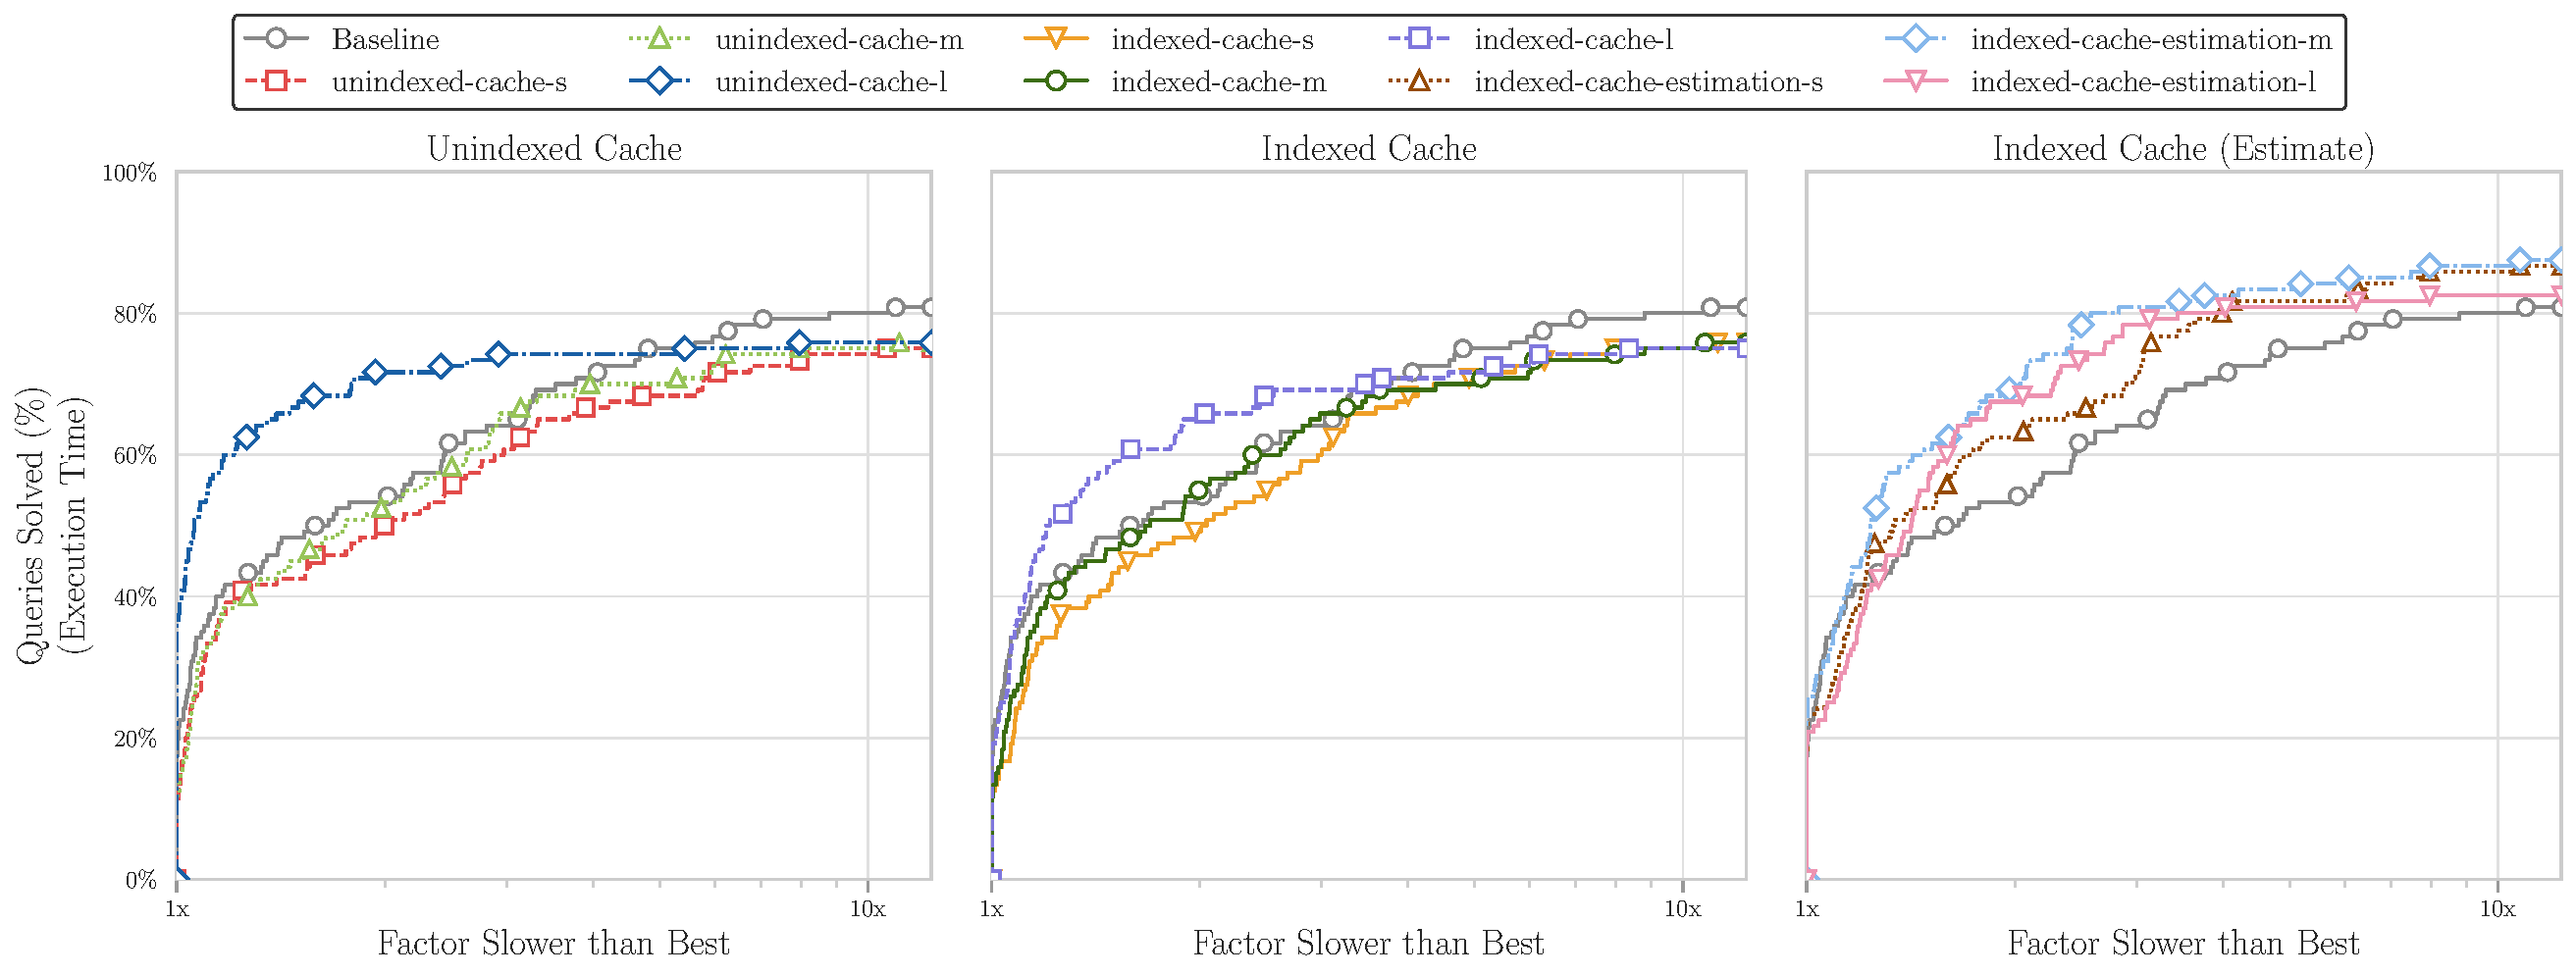
\includegraphics[width=\linewidth]{figures/performance_profile_random_sequences.pdf}
%     \caption{Performance profile of the tested cache algorithms on random query sequences.
%      The y-axis shows the percentage of queries that execute within 
%      a given performance factor (x-axis) of the fastest algorithm for that query.}
%     \label{fig:global_cache_performance_random_sequences}
% \end{figure*}

\paragraph{Scope and Limitations}
We evaluate SolidSessionBench against microbenchmarks and random sequences, 
but explicitly exclude hand-crafted scenarios and simple distributions.
Hand-crafted methods lack scalability, while simple distributions fail to capture complex user habits.
By automating logical sessions and user interests, our benchmark functions as a scalable superset of both approaches,
making direct comparison redundant. 
By contrast, the compared methods do not incorporate these sequence attributes, 
and our results show this omission risks drawing inaccurate conclusions.